% Track down:
% ASTR278 formula sheet
% ASTR378 formula sheet

% Formulae from:
% HSC + 
% Audrey's Sheets +
% Scifi Cheat Sheet

% MATH135 - no sheet
% MATH136 - no sheet
% MATH235 - no sheet
% PHYS107 + 2014 + 2017
% PHYS106 + 2014 + 2017
% PHYS201 + 2014 + 2017
% PHYS202 + 2015 + 2017
% PHYS301 + custom handwritten
% PHYS304 + custom Latex
% ASTR278 + 2015 + 2017
% ASTR377 + Lecture Slides
% ASTR378 + 2016 + 2017 + custom handwritten

% PHYS701 - custom handwritten - custom Latex
% PHYS702 - 2018 - 2018 integrals - custom handwritten

% ASTR707 - custom handwritten - exam sheets
% ASTR708 - custom handwritten - exam sheets

\documentclass[]{report}

%\usepackage{physics}
%\usepackage{mtpro2}

\usepackage[a4paper,top=2.0cm,bottom=2.0cm,left=2.0cm,right=2.0cm,marginparwidth=1.75cm]{geometry}
\usepackage{mathtools}
\usepackage{esint} 
\usepackage{fancyhdr}
\usepackage[colorlinks=true, allcolors=blue]{hyperref}
\usepackage{tikz}
\usepackage[
    type={CC},
    modifier={by-sa},
    version={4.0},
]{doclicense}
\usepackage{calligra}
\usepackage{wasysym}
\usepackage{times}

\urlstyle{same}

\DeclarePairedDelimiter\bra{\langle}{\rvert}
\DeclarePairedDelimiter\ket{\lvert}{\rangle}
\DeclarePairedDelimiterX\braket[2]{\langle}{\rangle}{#1 \delimsize\vert #2}
\DeclareMathAlphabet{\mathcalligra}{T1}{calligra}{m}{n}
\DeclareFontShape{T1}{calligra}{m}{n}{<->s*[2.2]callig15}{}

\newcommand \tab[1][1cm]{\hspace*{#1}}
\newcommand{\dn}[1]{\ \mathrm{d}#1}
\newcommand{\dd}[2]{ \dfrac{\dn #1}{\dn #2}}
\newcommand{\pp}[2]{\dfrac{\partial #1}{\partial #2}}
\newcommand{\curl}{\vec{\nabla}\times}
\newcommand{\divergence}{\vec{\nabla}\cdot}
\newcommand{\itemt}{\item \tab}
\newcommand{\items}{\item\ \ }
\newcommand{\degrees}{^{\circ}}
\newcommand{\scriptr}{\mathcalligra{r}\,}

\title{{\large A Web of Worlds presents} \ \\\ The Ultimate Cheat Sheet for Astrophysics Students}
\date{v 1.1 \\ \today}
\author{Lachlan Marnoch \\ \url{www.webofworlds.net}}

\begin{document}

\maketitle

\tableofcontents

%\twocolumn

\chapter{Physics}

	\section{Motion}

\subsection{Velocity}

\begin{itemize}
\itemt \( \vec{v} = \) \( \dfrac{\Delta \vec{x}}{\Delta t} = \dfrac{d \vec{x}}{dt} \) \(= \vec{\dot{x}}  \)
\end{itemize}

\subsection{Acceleration}

\begin{itemize}
\itemt \( \vec{a} = \dfrac{\Delta \vec{v}}{\Delta t} = \dfrac{d \vec{v}}{dt} = \dfrac{d^2 \vec{x}}{dt^2} = \vec{\ddot{x}}  \)	
\end{itemize}            
		
\subsection{Newton's Laws}

\subsubsection{Newton's First Law}
\begin{itemize}
\item When viewed in an inertial reference frame, an object either remains at rest or continues to move at a constant velocity, unless acted upon by a net force.
\end{itemize}

\subsubsection{Newton's Second Law}
\begin{itemize}
\itemt \(\vec{F}_{net} = m\vec{a} = \dd{\vec{p}}{t}	\)
\end{itemize}

\subsubsection{Newton's Third Law}
\begin{itemize}
\itemt \(\vec{F}_A = -\vec{F}_B	\) 
\item When one body exerts a force on a second body, the second body simultaneously exerts a force equal in magnitude and opposite in direction on the first body.
\end{itemize}			

\subsection{Momentum}
\begin{itemize}
\itemt \( \vec{p} = \gamma m\vec{v} \approx m\vec{v}\)
\itemt \( \Delta\vec{p} = \vec{F} \Delta t \)
\itemt \(\vec{F} = \dfrac{\Delta \vec{p}}{\Delta t} = \dd{\vec{p}}{t} \)
\end{itemize}

\subsection{Centripetal Force}
\begin{itemize}
\itemt \(F_c = \dfrac{mv^2}{r}\)
\end{itemize}		

\subsection{Kinetic Energy}	
\begin{itemize}
\itemt \( K = \frac{1}{2} mv^2 \)
\end{itemize}

\subsection{Projectile Motion}		
\begin{itemize}
\itemt \(v_y^2 = u_y^2 + 2a_y\Delta y \)
\itemt \( x = u_xt \)
\itemt \(\Delta y = u_y \Delta t + \frac{1}{2} a_y \Delta t^2 = u_y t + \frac{1}{2} \dfrac{F_{y}}{m} \Delta t^2\)
\end{itemize}	


\subsection{Rotation}

\subsubsection{Angular Velocity}
\begin{itemize}
\itemt \( \omega = \dd{\theta}{t} = \dot{\theta} \)
\itemt \( \omega = \dfrac{v}{r} \)
\itemt \( \vec{v} = \vec{r} \times \vec{\omega} \)
\end{itemize}

\subsubsection{Angular Acceleration}
\begin{itemize}
\itemt \( \alpha = \dd{\omega}{t} = \dd{^2\theta}{t^2} = \dot{\omega} = \ddot{\theta}\)
\end{itemize}

\subsubsection{Moment of Inertia}
\textit{Point Mass}
\begin{itemize}
\itemt \( I = mr^2 \)
\end{itemize}
\textit{Several Point Masses}
\begin{itemize}
\itemt \( I = \sum mr^2 \)
\end{itemize}
\textit{Continuous mass}
\begin{itemize}
\itemt \( I = \int r^2 \dn m \)
\end{itemize}
\textit{Parallel axis theorem}
\begin{itemize}
\itemt \( I = I_{com} + md^2 \)
\end{itemize}
\textit{Thin disc rotating about centre}
\begin{itemize}
\itemt \( I = \dfrac{MR^2}{2} \)
\end{itemize}
\textit{Thin hoop rotating about centre}
\begin{itemize}
\itemt \( I = MR^2 \)
\end{itemize}
\textit{Thin rod rotating about centre}
\begin{itemize}
\itemt \( I = \dfrac{ML^2}{12} \)
\end{itemize}
\textit{Thin rod rotating about end}
\begin{itemize}
\itemt \( I = \dfrac{ML^2}{3} \)
\end{itemize}


\subsubsection{Rotational Kinetic Energy}
\begin{itemize}
\itemt \( K_{rot} = \frac{1}{2} I \omega^2 \)
\end{itemize}

\subsubsection{Total Kinetic Energy}
\begin{itemize}
\itemt \( K_{tot} = K_{trans} + K_{rot} = \frac{1}{2} (mr_{com}^2 + I_{com})\omega^2 \)
\end{itemize}

\subsubsection{Angular Momentum}
\begin{itemize}
\itemt \( \vec{L} = I\vec{\omega} = \vec{r} \times \vec{p}\)
\end{itemize}

\subsubsection{Torque}
\begin{itemize}
\item \( \vec{\tau} = I\vec{\alpha} = \dd{L}{t} = \vec{r} \times \vec{F}\)
\end{itemize}

\subsection{Euler-Lagrange and the Hamiltonian}	

\subsubsection{Lagrangian}			
\begin{itemize}
\itemt \(\ell = T - V = \sum\limits_{lm} a(q)\dot{q}_l\dot{q}_m \)
\itemt \ \ \( = K(\dot{q}_l) - U(q_l)\)
\end{itemize}

\textit{Generalised coordinates \& momenta}
\begin{itemize}
\itemt \( p_k \equiv \pp{L}{\dot{q_k}}\)
\end{itemize}

\subsubsection{Euler-Lagrange Equation}			
\begin{itemize}
\itemt \( \dd{}{t} \pp{\ell}{\dot{x}} - \pp{\ell}{x} = 0\)
\end{itemize}

\subsubsection{Action}			
\begin{itemize}
\itemt \(S[x(t)] = \int\limits_{t_A}^{t_B} \ell(\dot{x}(t),x(t)) \dn t\)
\end{itemize}			

\subsubsection{Hamiltonian}
\begin{itemize}
\itemt \( \mathcal{H} = \sum\limits_{l} p_l \dot{q} - L \)
\itemt \( \dot{P} = -\dfrac{\partial H}{\partial Q} \)		
\itemt \( \dot{Q} = \dfrac{\partial H}{\partial P} \)
\itemt \( \dot{P} = -\omega^2Q \)
\itemt \(\dot{Q} = P\)
\end{itemize}
				
	\section{Oscillations}

\subsection{Springs}

\subsubsection{Force of a Spring}
\begin{itemize}
\itemt \(\vec{F} = -k_s\vec{x}\)
\end{itemize}

\subsubsection{Potential Energy of a Spring}
\begin{itemize}
\itemt \( U_s = \dfrac{1}{2} k_s x^2 \)
\end{itemize}

\subsubsection{Angular Frequency of a Spring}
\begin{itemize}
\itemt \( \omega = \sqrt{\dfrac{k_s}{m}} \)
\end{itemize}

	\section{Materials}

\subsection{Density}
\begin{itemize}
\itemt \( \rho = \dfrac{m}{V} = \dd{m}{V} \)
\end{itemize}
				
	\section{Energy}

\subsection{Work}
\begin{itemize}
\itemt \(W = \int\limits_{a}^{b} \vec{F}\cdot \dn\vec{l} \approx \vec{F} \cdot \vec{s}\)
\end{itemize}
				
	\section{Forces}

\subsection{Buoyancy (Archimedes' Principle)}			
\begin{itemize}
\itemt \( F_{buoy} = m_{displaced}g = \rho_{d} V_{d}g \)
\end{itemize}				

\subsection{Friction}			
\begin{itemize}
\itemt \( F_{K} \approx \mu_K F_\perp \)
\itemt \( F_{S} \leq \mu_S F_\perp \)
\end{itemize}				
				
	\section{Waves}
\begin{itemize}
\itemt \( a \sin(\omega t - kx + \phi) \)
\itemt \( k = \frac{2\pi}{\lambda} \)
\end{itemize}


\subsection{Wavelength}			
\begin{itemize}
\itemt \( v = f\lambda \)
\end{itemize}

\subsection{Angular Frequency}
\begin{itemize}
\itemt \( \omega = \dfrac{2\pi}{T} = 2\pi f \)
\end{itemize}

	\section{Newtonian Gravity}	

\subsection{Force of Gravity}
\begin{itemize}
\itemt \( \vec{F}_G = \dfrac{GmM}{r^2} \hat{r} = -m\vec{\nabla}\Phi(\vec{r}) \approx -mg\hat{y} = m\vec{g}\)
\end{itemize}	

\subsection{Gravitational Potential (potential energy per unit mass)}		
\begin{itemize}
\itemt \( \Phi(\vec{r}) = -\sum\limits_{i} \dfrac{GM(\vec{r}_i)}{|\vec{r}-\vec{r}_i|} = - \int \dfrac{G\mu(\vec{r'})}{|\vec{r} - \vec{r'}|} \dn^3\vec{r'} \)
\end{itemize}

\subsection{Gravitational field}
\begin{itemize}
\itemt \(\vec{g}(\vec{r}) = \dfrac{GM}{r^2} = -\nabla\Phi(\vec{r})\)
\end{itemize}										

\subsection{Gravitational Potential Energy}		
\begin{itemize}
\itemt \( U_G = -\dfrac{GmM}{r} \approx mgh\)
\end{itemize}

\subsection{Kepler's Third Law}		
\begin{itemize}
\itemt \( \dfrac{T^2}{r^3} = \dfrac{4\pi^2}{G(m+M)} = constant\)
\end{itemize}	

	\section{Electromagnetism}

		\subsection{Notation}
        \begin{itemize}
        \itemt \( \vec{\scriptr} = \vec{r} - \vec{r'} \)
        \end{itemize}

		\subsection{Maxwell's Equations}

\def\arraystretch{3}
\begin{tabular}{ |l|l|l| } 
\hline
					
  &	\textbf{Integral form}	& 	\textbf{Differential form}
\\ \hline

\textbf{Gauss's Law}	
&\( \oiint\limits_{S} \vec{E} \cdot \dn\vec{a} = \dfrac{1}{\varepsilon_0} \iiint\limits_V \rho \dn V \)	
& \( \divergence \vec{E} = \dfrac{\rho}{\varepsilon_0} \)
\\
& \hspace{1.4cm}\( = \dfrac{\sum Q_{enc}}{\varepsilon_0} \) &
\\ \hline

\textbf{Gauss's Law for Magnetism}	
&\( \oiint\limits_{S} \vec{B} \cdot \dn\vec{a} = 0 \)
&\( \divergence \vec{B} = 0 \)
\\ \hline

\textbf{Maxwell-Faraday equation}	
&\( \oint\limits_{b} \vec{E} \cdot \dn\vec{l} = -\dd{}{t} \iint\limits_S \vec{B} \cdot \dn\vec{a}\)	&\( \curl \vec{E} = -\pp{\vec{B}}{t} \)
\\ \hline

\textbf{Amp\'ere's circuital law}	
& \( \oint\limits_{b} \vec{B} \cdot \dn\vec{l} = \mu_0 \iint\limits_S \vec{J} \cdot \dn\vec{a} + \mu_0\varepsilon_0 \dd{}{t} \iint\limits_S \vec{E}\cdot d\vec{a}\)	
&\( \curl \vec{B} = \mu_0(\vec{J} + \varepsilon_0 \pp{\vec{E}}{t}) \)
\\
& \hspace{1.1cm} \( = \mu_0 (I_{enc} + \varepsilon_0 \dd{}{t} \int\limits_S \vec{E} \cdot \dn\vec{a} ) \) &
\\ \hline
\end{tabular}

%\twocolumn

		\subsection{Lorentz Force}

\subsubsection{On a point charge}
\begin{itemize}
\itemt \( \vec{F} = q(\vec{E}+\vec{v}\times \vec{B})\)
\end{itemize}

\subsubsection{On a current}
\begin{itemize}
\itemt \( \dn\vec{F} = I \int \dn\vec{l} \times \vec{B} \)
\itemt \( \vec{F} = \vec{I}L\times \vec{B} \)
\end{itemize}

		\subsection{Electric Field}
        
\begin{itemize}
\itemt \( \vec{E} = \int\limits_V \dfrac{\rho(\vec{r'})}{\scriptr ^2}\hat{\scriptr} \dn\tau \)
\end{itemize}

\subsubsection{From a single point charge}
\begin{itemize}
\itemt \( \vec{E} = \dfrac{1}{4\pi\varepsilon_0} \dfrac{q}{r^2} \hat{r} \)
\end{itemize}

\subsubsection{From a dipole}
\begin{itemize}
\itemt \( |\vec{E}_axis| \approx \dfrac{2p}{4\pi\varepsilon_0r^3} \)
\itemt \( |\vec{E}_\perp| \approx \dfrac{p}{4\pi\varepsilon_0r^3} \)
\end{itemize}

		\subsection{Dipole moment}
        
\begin{itemize}
\itemt \( \vec{p} = q\vec{d} \)
\end{itemize}

		\subsection{Electric potential}
        
\begin{itemize}
\itemt \( V = \dfrac{1}{4\pi\varepsilon_0} \dfrac{Q}{\scriptr} \)
\itemt \( \nabla^2 V = \dfrac{-\rho}{\varepsilon_0} \)
\end{itemize}

\subsubsection{In a single-point charge field}
\begin{itemize}
\itemt \( \Delta (\vec{r}) = \dfrac{1}{4\pi\varepsilon_0}\dfrac{q}{r} \)
\end{itemize}
        
        \subsection{Electric potential difference}
        
\begin{itemize}
\itemt \( \Delta (\vec{r}) = - \int\limits_{\vec{b}}^{\vec{a}} \vec{E}\cdot\dn \vec{l} \)
\end{itemize}

\subsubsection{In a single-point charge field}
\begin{itemize}
\itemt \( \Delta (\vec{r}) = \dfrac{1}{4\pi\varepsilon_0} Q (\dfrac{1}{b} - \dfrac{1}{a}) \)
\end{itemize}

		\subsection{Electric potential energy}
        
\begin{itemize}
\itemt \( U_E = q\Delta V = \dfrac{1}{4\pi \varepsilon_0} \dfrac{qQ}{\scriptr} \)
\end{itemize}

\subsubsection{Energy stored in an electrostatic field distribution}
\begin{itemize}
\itemt \( U_E = \frac{1}{2} =\epsilon_0 E^2 \times volume \)
\end{itemize}

		\subsection{Charge densities}
        
\subsubsection{Surface}
\begin{itemize}
\itemt \( \sigma = \dd{q}{a} = \dfrac{Q}{A} \)
\end{itemize}
\subsubsection{Line}
\begin{itemize}
\itemt \( \lambda = \dd{q}{l} = \dfrac{Q}{L} \) 
\end{itemize}

		\subsection{Current densities}
        
\subsubsection{Volume}
\begin{itemize}
\itemt \( \vec{J} = \dd{\vec{I}}{\vec{a}_\perp} = \dfrac{I}{A_\perp} = \sigma(\vec{E}+\vec{v}\times B) = |q|nu (\vec{E}+\vec{v}\times B)\)
\itemt \( \vec{\nabla} \cdot \vec{J} = 0 \)
\end{itemize}

\subsubsection{Surface}
\begin{itemize}
\itemt \( \vec{K} = \dd{\vec{I}}{\vec{l}_\perp} = \dfrac{I}{l} = \sigma \vec{v}\)
\end{itemize}




		\subsection{Circuits}

\subsubsection{Electron drift velocity}
\begin{itemize}
\itemt \( \bar{v} = u\vec{E}_{net} \)
\end{itemize}	

\subsubsection{Current per unit charge}
\begin{itemize}
\itemt \(i = nA_{cs}\bar{v} = nA_{cs}uE_{net}\)
\end{itemize}

\subsubsection{Current}
\begin{itemize}
\itemt \( I = ei = enA_{cs}uE_{net} = \dd{q}{t}\)
\end{itemize}	

\subsubsection{Electrical Power}
\begin{itemize}
\itemt \( P = IV = I^2R \)
\end{itemize}

\subsubsection{Voltage (Electric potential difference)}
\begin{itemize}
\itemt \( V = \Delta V = IR = - \varepsilon \)
\end{itemize}

\subsubsection{Electromotive Force (EMF) from a Non-Coulomb force}
\begin{itemize}
\itemt \( \epsilon = \dfrac{F_{NC}d}{e} \)
\end{itemize}

\subsubsection{Resistance}
\begin{itemize}
\itemt \( R = \dfrac{L\rho}{A} = \dfrac{L}{\sigma A} \)					
\itemt \( R_{series} = R_1 + R_2 + ... +R_n \)
\itemt \( \dfrac{1}{R_{parallel}} = \dfrac{1}{R_1} + \dfrac{1}{R_2} + ... + \dfrac{1}{R_n} \)
\end{itemize}

		\subsection{Capacitors}

\subsubsection{Capacitance}
\begin{itemize}
\itemt \( C = \dfrac{Q}{V} = \dfrac{\varepsilon A}{d} = \dfrac{k\varepsilon_0A}{d} \)
\end{itemize}

\subsubsection{Energy stored in a capacitor}
\begin{itemize}
\itemt \( W = \dfrac{CV^2}{2} \)
\end{itemize}

\subsubsection{Electric field in a capacitor}
\begin{itemize}
\itemt \( E = \dfrac{Q}{\varepsilon_0 A} \)
\end{itemize}

\subsubsection{Potential difference across a capacitor}
\begin{itemize}
\itemt \( \Delta V = -\dfrac{dQ}{A\varepsilon_0} \)
\end{itemize}
				
		\subsection{Magnetic fields}
        
\begin{itemize}
\itemt \( \vec{B}(\vec{\scriptr}) = \dfrac{\mu_0}{4\pi} \int \dfrac{\vec{I}\times\hat{\scriptr}}{\scriptr^2} \dn l \)
\itemt \( \dn \vec{B} = \dfrac{\mu_0}{4\pi} \dfrac{q\vec{v}\times\hat{\scriptr}}{\scriptr^2} = \dfrac{\mu_0}{4\pi} \dfrac{I\dn\vec{l}\times\hat{\scriptr}}{\scriptr^2} \)
\end{itemize}

\subsubsection{Magnetic field due to a wire}
\begin{itemize}
\itemt \( \vec{B} = \dfrac{\mu_0}{4\pi} \dfrac{2I}{r} \hat{\phi} \)
\end{itemize}

\subsubsection{Magnetic vector potential}
\begin{itemize}
\itemt \( \vec{A}(\vec{\scriptr}) = \dfrac{\mu_0}{4\pi} \int \dfrac{\vec{J}(\vec{r'})}{\scriptr} \dn \tau \)
\itemt \( \curl\vec{A} = \vec{B} \)
\itemt \( \vec{\nabla} \times (\vec{\nabla} \times \vec{A}) = -\mu_0 \vec{J} \)
\itemt \( \divergence\vec{A} = 0 \)
\end{itemize}

		\subsection{Inductors}
        
\begin{itemize}
\itemt \( \varepsilon = - LI \)
\end{itemize}
        
\subsubsection{Energy stored in an inductor}  
\begin{itemize}
\itemt \( W = \dfrac{LI^2}{2} \)
\end{itemize}

		\subsection{Materials}

\subsubsection{Macroscopic Maxwell's Equations (Materials)}

\def\arraystretch{2.5}
\begin{tabular}{ |l|l|l| } 
\hline
					
  &	\textbf{Integral form}	& 	\textbf{Differential form}
\\ \hline

\textbf{Gauss's Laws}	
&\( \oiint\limits_{S} \vec{P} \cdot \dn\vec{a} = -\sum Q_B \)	
& \( \divergence \vec{P} = -\rho_B \)
\\
& \( \oiint\limits_{S} \vec{D}\cdot\dn\vec{a} = \sum Q_f \) 
& \( \divergence \vec{D} = \rho_f \)
\\ \hline

\textbf{Gauss's Law for Magnetism}	
&\( \oiint\limits_{S} \vec{B} \cdot \dn\vec{a} = 0 \)
&\( \divergence \vec{B} = 0 \)
\\ \hline

\textbf{Maxwell-Faraday equation}	
&\( \oint\limits_{b} \vec{E} \cdot \dn\vec{l} = -\dd{}{t} \iint\limits_S \vec{B} \cdot \dn\vec{a}\)	
&\( \curl \vec{E} = -\pp{\vec{B}}{t} \)
\\ \hline

\textbf{Amp\'ere's circuital law}	
& \( \oint\limits_{b} \vec{H} \cdot \dn\vec{l} = I_{f,enc} + \pp{}{t} \iint\limits_S \vec{D}\cdot \dn \vec{a}\)	
&\( \curl \vec{H} = \vec{J_f} + \pp{\vec{D}}{t} \)
\\ \hline
\end{tabular}


\subsubsection{Dielectric constant}
\begin{itemize}
\itemt \( k = \dfrac{\varepsilon}{\varepsilon_0} = \varepsilon_r \)
\itemt \( \varepsilon = k\varepsilon_0 = \varepsilon_r \varepsilon\)
\end{itemize}

\subsubsection{Susceptibility}
\begin{itemize}
\itemt \( \chi_e = 1-\varepsilon_r \)
\end{itemize}

\subsubsection{Polarisability}
\begin{itemize}
\itemt \( \vec{P} = \varepsilon_0\chi_e\vec{E} = n\vec{p} \)
\end{itemize}

\subsubsection{Bound Charge}
\begin{itemize}
\item[Surface] 
\itemt \( \sigma_B = \vec{p}\cdot\hat{n} \)
\item[Volume]
\itemt \( \rho_B = -\vec{\nabla}\cdot\vec{P} \)
\item[Total]
\itemt \( Q_B = \sigma_B + \rho_B = \vec{p}\cdot\hat{n} -\vec{\nabla}\cdot\vec{P} \)
\end{itemize}

\subsubsection{Electric displacement}
\begin{itemize}
\itemt \( \vec{D} = \varepsilon \vec{E} = k\varepsilon_0 \vec{E} = \varepsilon_0\vec{E} + \vec{P} \)
\end{itemize}

\subsubsection{Magnetic field}
\begin{itemize}
\itemt \( \vec{H} = \dfrac{\vec{B}}{\mu_0} - \vec{M} \)
\end{itemize}

\subsubsection{Magnetic dipole}
\begin{itemize}
\itemt \( \vec{m} = I\vec{a} \)
\end{itemize}

\subsubsection{Bound current}
\begin{itemize}
\itemt \( \vec{J}_B = \curl \vec{M} \)
\itemt \( \vec{K}_B = \vec{M}\times\hat{n} \)
\end{itemize}


	\section{Special Relativity}

\subsection{Interval}
\begin{itemize}
\itemt \( \Delta s^2 = -c^2\Delta t^2 + \Delta x^2 +\Delta y^2 +\Delta z^2 \)
\itemt \( \dn s^2 = -c^2\dn t^2 + \dn x^2 + \dn y^2 + \dn z^2 \)
\itemt \( \Delta s^2 < 0 \) is a timelike interval. Events separated by this interval can be causally related.
\itemt \( \Delta s^2 = 0 \) is a lightlike interval. Events separated by this interval can be causally related, but only by a lightspeed signal.
\itemt \( \Delta s^2 > 0 \) is a spacelike interval. Events separated  by this interval CANNOT be causally related.
\end{itemize}

\subsubsection{Gamma Factor}		
\begin{itemize}
\itemt \( \gamma = \dfrac{1}{\sqrt{1-(\dfrac{v}{c})^2}} \)
\itemt \( \gamma = \dfrac{dt}{d\tau} \)
\end{itemize}		

\subsubsection{Mass-energy}
\begin{itemize}
\itemt \( E_{rest} = mc^2\)
\itemt \( E = \gamma mc^2 = \dfrac{1}{\sqrt{1-(\dfrac{v}{c})^2}}mc^2 \)
\end{itemize}

\subsubsection{Relativistic kinetic energy}
\begin{itemize}
\itemt \( K = \gamma mc^2 - mc^2 \)
\end{itemize}

\subsubsection{Length contraction}
\begin{itemize}
\itemt \( l_v = \dfrac{l_0}{\gamma} = l_0\sqrt{1-(\dfrac{v}{c})^2} \)
\end{itemize}

\subsubsection{Time dilation}
\begin{itemize}
\itemt \( t_v = \gamma t_0 = \dfrac{t_0}{\sqrt{1-(\dfrac{v}{c})^2}}\)
\end{itemize}

\subsubsection{Mass dilation}
\begin{itemize}
\itemt \( m_v = \gamma m_0 = \dfrac{m_0}{\sqrt{1-(\dfrac{v}{c})^2}}\)
\end{itemize}

\subsubsection{Relative Velocity}
\begin{itemize}
\itemt \( u_x'= \dfrac{\Delta x'}{\Delta  t} = \dfrac{u_x-v_x}{1-\dfrac{v_xu_x}{c^2}} \)
\end{itemize}

\subsubsection{Relativistic Momentum}
\begin{itemize}
\itemt \( \vec{p} = \gamma \vec{v} = \dfrac{m\vec{v}}{\sqrt{1-(v/c)^2}} \)
\end{itemize}

\subsection{Four-vectors}
\def\arraystretch{1}
\subsubsection{Four-space}			
\begin{itemize}
\itemt \(\mathbf{s} = \mathbf{x} = 
\begin{bmatrix}
ct \\
x \\
y \\
z \\
\end{bmatrix}
\)
\end{itemize}

\subsubsection{Four-velocity (proper velocity)}			
\begin{itemize}
\itemt \(\textbf{u} = \dfrac{d\textbf{s}}{d\tau} = \gamma 
\begin{bmatrix} 
c \\
v_x\\
v_y\\
v_z
\end{bmatrix}\)
\itemt \( \textbf{u}\cdot\textbf{u} = -c^2  \)
\end{itemize}

\subsubsection{Four-acceleration}			
\begin{itemize}
\itemt \(\textbf{w} = \dfrac{d\textbf{u}}{d\tau} = \gamma 
\begin{bmatrix} 
c \\
v_x\\
v_y\\
v_z
\end{bmatrix}\)
\item \( \textbf{w}\cdot\textbf{u} = 0 \)
\end{itemize}

\subsubsection{Four-momentum}			
\begin{itemize}
\itemt \(\textbf{p} = 
\begin{bmatrix} 
E/c \\
p_x\\
p_y\\
p_z
\end{bmatrix} = \gamma m
\begin{bmatrix} 
c \\
v_x\\
v_y\\
v_z
\end{bmatrix} = m\textbf{u}\)
\end{itemize}	
                
\subsection{Frames of Reference}		

\subsubsection{Condition for an inertial frame}	
\begin{itemize}
\itemt \( \dfrac{d^2 x}{dt^2} = \dfrac{d^2 y}{dt^2} = \dfrac{d^2 z}{dt^2} \) \normalsize \(= 0\)
\end{itemize}		 

\subsubsection[GT]{Galilean Transformations}				 
\begin{itemize}
\itemt \(x' = x + vt\)
\itemt \(y' = y\)
\itemt \(z' = z\)
\itemt All assuming $x$ is along the axis of motion and \textit{x = x'} when $t = 0$.	
\end{itemize}

\subsubsection{Lorentz Boosts}				
\begin{itemize}
\itemt \( \ t' = \gamma (t-\dfrac{vx}{c^2})\)
\itemt \( x' = \gamma (x-vt)\)
\itemt \( y' = y \)
\itemt \( z' = z \)
\itemt ($x$ is along the axis of motion)					
\itemt \(					
\begin{bmatrix}
ct' \\
x' \\
y' \\
z' \\
\end{bmatrix} =
\begin{bmatrix}
\gamma 		&-v\gamma	&0	&0 	\\
-v\gamma 	&\gamma		&0	&0	\\
0 			&0			&1	&0	\\
0 			&0			&0	&1	\\
\end{bmatrix}
\begin{bmatrix}
ct \\
x \\
y \\
z \\
\end{bmatrix} \)
\end{itemize}		

\subsubsection{General Lorentz transformation}
\begin{itemize}
\itemt 
\( \begin{bmatrix}
b'^0 \\
b'^1 \\
b'^2 \\
b'^3 \\
\end{bmatrix} =
\begin{bmatrix}
\gamma 		&-v\gamma	&0	&0 	\\
-v\gamma 	&\gamma		&0	&0	\\
0 			&0			&1	&0	\\
0 			&0			&0	&1	\\
\end{bmatrix}
\begin{bmatrix}
b^0 \\
b^1 \\
b^2 \\
b^3 \\
\end{bmatrix} \)
\itemt Motion along the $x$-axis.
\end{itemize}


\subsubsection{Proper Time}
\begin{itemize}
\itemt \( \tau = \int\limits_{t_A}^{t_B} \dfrac{1}{\gamma} \dn t =\int\limits_{t_A}^{t_B} \sqrt{1 - \dfrac{{v}^2(t)}{c^2}} \dn t \)
\end{itemize}

	\section{General Relativity}
    
		\subsection{Metrics}

\subsubsection{Minkowski}
\begin{itemize}
\itemt \( \eta =
\begin{bmatrix}
-1 	&0	&0	&0 	\\
0 	&1	&0	&0	\\
0 	&0	&1	&0	\\
0 	&0	&0	&1	\\
\end{bmatrix} =
\begin{bmatrix}
-1 	&0	&0	&0 	\\
0 	&1	&0	&0	\\
0 	&0	&r^2	&0	\\
0 	&0	&0	&r^2 \sin^2 \theta	\\
\end{bmatrix}\)
\itemt \( \dn s^2 = -c^2 \dn t^2 + \dn x^2 + \dn y^2 + \dn z^2 \tab[0.5cm]=  -c^2 \dn t^2 + \dn r^2 + r^2 \dn \theta ^2 + r^2 \sin^2 \theta \dn \phi^2 \)
\end{itemize}

\subsubsection{Schwarzschild}
\begin{itemize}
\itemt \( g =
\begin{bmatrix}
-(1-\dfrac{2GM}{c^2r}) 	&0							&0		&0 					\\
0 						&(1-\dfrac{2GM}{c^2r})^{-1}	&0		&0					\\
0 						&0							&r^2	&0					\\
0 						&0							&0		&r^2\sin^2\theta	\\
\end{bmatrix} \)
\itemt \( \dn s^2 = -(1-\dfrac{2GM}{c^2r})c^2 \dn t^2 + (1-\dfrac{2GM}{c^2r})^{-1} \dn r^2 + r^2 \dn \theta^2 + r^2\sin^2 \theta \dn \phi^2) \)
\end{itemize}

		\subsection{Rindler coordinates}

\subsubsection{Line element}
\begin{itemize}
\itemt \( \dn s^2 = -(1+\dfrac{gx'}{c^2})^2(c \dn t')^2 + \dn x' \)
\end{itemize}

		\subsection{Einstein summation notation}
        
\begin{itemize}
\item \( a_\mu b^\mu \equiv \sum\limits^3_{\mu=0} a_\mu b^\mu \)
\item Contravariant: $e^\alpha$
\item Covariant: $e_\alpha$
\itemt \( t_{\alpha\beta} = g_{\beta\gamma} t_\alpha{}^\gamma \)
\itemt \( t_\alpha{}^\beta = g^{\beta\gamma} t_{\alpha\gamma} \)
\itemt \( t'^\alpha{}_\beta = \pp{x'^\alpha}{x^\gamma} \pp{x^\delta}{x'^\beta} t^\gamma{}_\delta\)
\itemt \( t'_\alpha{}^\beta = \pp{x^\gamma}{x'^\alpha} \pp{x'^\beta}{x^\delta} t_\gamma{}^\delta\)
\end{itemize}

\subsubsection{Metrics}
\begin{itemize}
\itemt \( \dn s^2 = g_{\alpha\beta} \dn x^\alpha \dn x^\beta \)
\itemt \( g^{\alpha\beta} = \dfrac{1}{g_{\alpha\beta}} \)
\itemt \( \delta^\alpha_\beta =
\begin{cases}
      1 & \alpha = \beta \\
      1	& \alpha \neq \beta \\
\end{cases}
\)
\itemt \( \delta^\alpha_\gamma a^\gamma = a^\alpha \)
\itemt \( g^{\alpha\gamma}g_{\gamma\beta} = \delta^\alpha_\beta \) % And the reverse?
\end{itemize}

\subsubsection{Four-vector product}
\begin{itemize}
\itemt \( \textbf{a}\cdot \textbf{b} = g_{\alpha\beta}a^\alpha b^\beta = a_\beta b^\alpha\)
\end{itemize}
        
		\subsection{Christoffel symbols}

\begin{itemize}
\itemt \( \Gamma^\alpha{}_{\beta\gamma} = \frac{1}{2} g^{\alpha\delta} (\pp{g_{\delta\beta}}{x^\gamma} + \pp{g_{\delta\gamma}}{x^\beta} - \pp{g_{\beta\gamma}}{x^\delta})  \) 

\itemt \( \Gamma_{\alpha\beta\gamma} = \frac{1}{2}(\pp{g_{\delta\beta}}{x^\gamma} + \pp{g_{\delta\gamma}}{x^\beta} - \pp{g_{\beta\gamma}}{x^\delta})  \) 

\itemt \( \dd{^2 x^\mu}{\tau} + \Gamma^\mu{}_{\alpha\beta} \dd{x^\alpha}{\tau} \dd{x^\beta}{\tau} = 0\)
\end{itemize}

		\subsection{Covariant derivatives}
\begin{itemize}
\itemt \( \nabla_\gamma t^\alpha{}_\beta = \pp{t^\alpha{}_\beta}{x^\gamma} + \Gamma^\alpha{}_{\gamma\delta}t^\delta{}_\beta - \Gamma^\delta{}_{\gamma\beta}t^\alpha{}_\delta \)

\itemt \( \nabla_\gamma t^{\alpha\beta} = \pp{t^{\alpha\beta}}{x^\gamma} + \Gamma^\alpha{}_{\gamma\delta}t^{\delta\beta} + \Gamma^\beta{}_{\gamma\delta}t^{\alpha{}\delta} \)

\itemt \( \nabla_\gamma t_{\alpha\beta} = \pp{t_{\alpha\beta}}{x^\gamma} - \Gamma^\delta{}_{\gamma\alpha}t_{\delta\beta} - \Gamma^\delta{}_{\gamma\beta}t^{\alpha\delta} \)

\itemt \( \nabla_\gamma t_\alpha{}^\beta = \pp{t_\alpha{}^\beta}{x^\gamma} - \Gamma^\delta{}_{\gamma\alpha}t_\delta{}^\beta + \Gamma^\beta{}_{\gamma\delta}t_\alpha{}^\delta \)
\end{itemize}

		\subsection{Riemann curvature tensor}
\begin{itemize}
\itemt \( R^\alpha{}_{\beta\gamma\delta} = \pp{\Gamma^\alpha{}_{\beta\delta}}{x^\gamma} - \pp{\Gamma^\alpha{}_{\beta\gamma}}{x^\delta} + \Gamma^\alpha{}_{\gamma\epsilon}\Gamma^\epsilon{}_{\beta\delta} - \Gamma^\alpha{}_{\delta\epsilon}\Gamma^\epsilon{}_{\beta\gamma} \)

\itemt \( R_{\alpha\beta\gamma\delta} = \frac{1}{2}(\pp{^2g_{\alpha\delta}}{x^\beta \partial x^\gamma} - \pp{^2g_{\alpha\gamma}}{x^\beta \partial x^\delta} - \pp{^2g_{\beta\delta}}{x^\alpha \partial x^\gamma}) + \pp{^2g_{\beta\gamma}}{x^\alpha \partial x^\delta}\)

\itemt \( R_{\alpha\beta\gamma\delta} = -R_{\beta\alpha\gamma\delta} \)
\itemt \( R_{\alpha\beta\gamma\delta} = -R_{\beta\alpha\delta\gamma} \)
\itemt \( R_{\alpha\beta\gamma\delta} = R_{\delta\gamma\alpha\beta} \)
\itemt \( R_{\alpha\beta\gamma\delta} + R_{\alpha\delta\beta\gamma} + R_{\alpha\gamma\delta\beta = 0}\)

\end{itemize}

		\subsection{Ricci curvature tensor}
\begin{itemize}
\itemt \( R_{\alpha\beta} = R^\gamma{}_{\alpha\gamma\beta} \)
\itemt \( R = R^\alpha{}_\alpha  \)
\end{itemize}


		\subsection{Einstein's equations}
\begin{itemize}
\itemt \( R_{\mu\nu} - \frac{1}{2} g_{\mu\nu} R + \Lambda g_{\mu\nu}= \dfrac{8\pi G}{c^4} T_{\mu\nu} \)
\end{itemize}

	\section{Thermodynamics}



\subsection{Ideal Gases}

\subsubsection{Ideal Gas Law}
\begin{itemize}
\itemt \( pV = Nk_BT \)
\end{itemize}

\subsubsection{Heat / Thermal Energy}
\begin{itemize}
\itemt \( Q = mc \Delta T \)
\end{itemize}

\subsubsection{Heat Capacity}
\begin{itemize}
\itemt \( C = \dd{Q}{T} \)
\end{itemize}

\subsubsection{Specific Heat Capacity}
\begin{itemize}
\itemt \( c = \dfrac{C}{m} \)
\end{itemize}





\subsection{Microstates}

\begin{itemize}
\itemt \( \Omega = \dfrac{(q+N-1)}{q!(N-1)} \)
\end{itemize}

\subsection{Entropy}

\begin{itemize}
\itemt \( S = k_B \ln \Omega \)
\end{itemize}


\subsection{Black bodies}

\subsubsection{Energy of a photon}
% This might not be the best place for this
\begin{itemize}
\itemt \( E = hf \)
\end{itemize}

\subsubsection{Wien's Displacement Law}
\begin{itemize}
\itemt \( \lambda_{max} = \dfrac{b}{T} = (2.8977729\times10^{-3}) \dfrac{1}{T} \)
\end{itemize}

\subsubsection{Stefan-Boltzmann Law}
\begin{itemize}
\itemt \( I = \sigma T^4 \)
\end{itemize}

\subsubsection{Spectrum}
\begin{itemize}
\itemt \( B_\lambda (T) = \dfrac{2 h c^2}{\lambda^5} \dfrac{1}{\exp(\dfrac{h c}{\lambda k_B T} - 1)} \)
\itemt \( B_\nu (T) = \dfrac{2 h \nu}{c^2} \dfrac{1}{\exp(\dfrac{h \nu}{k_B T}) - 1} \)
\end{itemize}

	\section{Quantum Mechanics}	

\subsection{The Uncertainty Principle}
\begin{itemize}
\item \( \Delta x \Delta p \geq \dfrac{\hbar}{2} \)
\item \( \Delta E \Delta t \geq \dfrac{\hbar}{2} \)
\end{itemize}

\subsection{Bras and Kets}			
\begin{itemize}
\itemt \( \ket{\psi} = \bra{\psi}^\dagger \)
\end{itemize}				

\subsection{Rules for an Inner Product}			

\begin{itemize}
\itemt \( \braket{\psi}{\phi} \equiv (\ket{\psi}, \ket{\phi}) \)
\item Symmetric:
\subitem \( \braket{\psi}{\phi} = \braket{\phi}{\psi}^* \)
\item Linear in second component
\item Anti-linear in first component
\end{itemize}				

\subsection{The Born Rule}
\begin{itemize}
\itemt \( P = |\braket{\psi}{\psi}|^2 \)
\end{itemize}

\subsection{Expectation}
\begin{itemize}
\itemt \( \langle A \rangle = \int A |\Psi(x,t)|^2 \dn x \)
\itemt \( \langle A \rangle = \bra{\psi} A \ket{\psi} \)
\end{itemize}	

\subsection{Variance}
\begin{itemize}
\itemt \( \mathrm{var}(A) = \bra{\psi} A^2 \ket{\psi} - \bra{\psi} A \ket{\psi}^2 \)
\end{itemize}	

\subsection{Standard Deviation}
\begin{itemize}
\itemt \( \delta A = \sqrt{\mathrm{var}(A)} = \sqrt{\bra{\psi} A^2 \ket{\psi} - \bra{\psi} A \ket{\psi}^2} \)
\end{itemize}

\subsection{Trace}
\begin{itemize}
\itemt \( \mathrm{Tr} (A) = \sum\limits_{j} \bra{x_j} A \ket{x_j} \)
\end{itemize}

\subsection{Partial Trace}			
\begin{itemize}
\itemt \( Tr_B(\ket{a}\bra{a}\otimes\ket{b}\bra{b}) \equiv \ket{a}\bra{a} \mathrm{Tr} (\ket{b}\bra{b}) \)
\itemt \( \mathrm{Tr} (k_{AB}) = Tr_A(Tr_B(k_{AB})) = Tr_B(Tr_A(k_{AB})) \)
\itemt \( \rho_B = Tr_A(\rho_{AB}) \)
\itemt The partial trace is linear
\end{itemize}

\subsection{The Schr\"odinger Equation}			
\begin{itemize}
\itemt \( i \hbar \dfrac{\partial }{\partial t} \Psi (r,t) = \hat{H} \Psi(r,t) \)
\itemt \( -\dfrac{\hbar^2}{2m} \pp{^2 \Psi(x,t)}{x^2} + V(x)\Psi(x,t) = i\hbar\pp{\Psi(x,t)}{t} \)
\itemt \( -\dfrac{\hbar^2}{2m} \pp{^2 \psi(x)}{x^2} + V(x)\psi(x,t) = E\psi(x) \)
\itemt \( \hat{H}\ket{\Psi(t)} = i\hbar \dfrac{\partial }{\partial t} \ket{\Psi(t)} \)
\end{itemize}

\subsection{Heisenberg equation of motion}			
\begin{itemize}
\itemt \( \dfrac{d}{dt} \hat{A}(t) = \dfrac{i}{\hbar}[\hat{H},\hat{A}(t)] \)
\end{itemize}			

\subsection{Operators}			
\begin{itemize}
\itemt \( a_{jk} = \bra{j} A \ket{k} \)
\end{itemize}			

\subsubsection{Diagonalizable Operator}			
\begin{itemize}
\itemt \( A = \sum\limits_{j} \lambda_j \ket{\lambda_j} \bra{\lambda_j} \)
\end{itemize}

\subsubsection{Normal Operator}			
\begin{itemize}
\itemt \( A =\sum\limits_{j} \ket{\lambda_j} \bra{\lambda_j} \)
\end{itemize}

\subsubsection{Eigenstate Operators}			
\begin{itemize}
\itemt \( (\ket{\lambda_k}\bra{\lambda_k})^n = \ket{\lambda_k}\bra{\lambda_k} \)
\end{itemize}

\subsubsection{Identity}
\begin{itemize}
\itemt \( I = \sum\limits_{j} \ket{x_j} \bra{x_j} \)
\end{itemize}

\subsubsection{Projector}
\begin{itemize}
\itemt \( P = \ket{\psi} \bra{\psi} \)
\end{itemize}				

\subsubsection{Density operator}
\begin{itemize}
\itemt \( \rho \equiv \sum\limits_{j} P_j \ket{\psi_j}\bra{\psi_j} \)
\itemt Hermitian: \( \rho^\dagger = \rho \)
\itemt Normalised: \( \mathrm{Tr} (\rho) = 1 \)
\itemt Positive Semi-Definite: \( \bra{\psi}\rho\ket{\psi} \geq 0, \ \forall \ \ket{\psi} \in \mathbf{H} \)
%\item $\rho' = U\rho U^\dagger$
\itemt \( purity = \mathrm{Tr} (\rho^2) \)
	\begin{itemize}
	\itemt \( \dfrac{1}{d} \leq \mathrm{Tr} (\rho^2) \leq 1 \)
	\itemt Pure: \( \mathrm{Tr} (\rho^2) = 1 \)
	\itemt Maximally mixed: \( \mathrm{Tr} (\rho^2) = \dfrac{1}{d} \)
	\end{itemize}
\itemt \( \rho_A = Tr_B(\rho_{AB}) \)
\itemt \( \langle A\rangle = \mathrm{Tr} (\rho A) \)
\end{itemize}				

\subsubsection{Pauli Operators}
\begin{itemize}
\itemt \( \sigma_x = X = \ket{0}\bra{1} + \ket{1}\bra{0} \doteq 		
\begin{bmatrix}
0 & 1 \\
1 & 0
\end{bmatrix} \)					
\itemt \( \sigma_y = Y = i\ket{1}\bra{0} - i\ket{0}\bra{1} \doteq 
\begin{bmatrix}
0 & -i \\
i & 0
\end{bmatrix} \)					
\itemt \( \sigma_z = Z = \ket{0}\bra{0} - \ket{1}\bra{1} \doteq 
\begin{bmatrix}
1 & 0 \\
0 & -1
\end{bmatrix} \)					
\itemt \( I = \ket{0}\bra{0} + \ket{1}\bra{1} \doteq \begin{bmatrix}
1 & 0 \\
0 & 1
\end{bmatrix} \) (Sometimes included)					
\itemt \( Trx = \mathrm{Tr} (Y) = \mathrm{Tr} (Z) = 0 \)					
\itemt With respect to Hilbert-Schmidt Inner Product:
\subitem \( ||X|| = ||Y|| = ||Z|| = ||I|| = \sqrt{2} \)				
\end{itemize}

\textit{Properties}
\begin{itemize}
\itemt Unitary
\itemt Hermitian
\itemt \( \lambda = \pm 1 \)
\end{itemize}

\subsubsection{Photon Annihilation and Creation Operators}			
\begin{itemize}
\itemt \( \hat{a}\ket{n} = \sqrt{n}\ket{n-1} \)
\itemt \( \hat{a}^\dagger\ket{n} = \sqrt{n+1}\ket{n+1} \)
\itemt \( \hat{a}\ket{\alpha} = \alpha\ket{\alpha} \)
\itemt \( \bra{\alpha}\hat{a}^\dagger = \alpha^*\bra{\alpha} \)
\end{itemize}

\subsubsection{Atomic Energy Level Operators (for a two-level approximation)}	
\begin{itemize}
\itemt \( \hat{\sigma}_+ = \ket{e}\bra{g} \)
\itemt \( \hat{\sigma}_- = \ket{g}\bra{e} \)
\itemt \( \hat{\sigma}_z = \ket{e}\bra{e} - \ket{g}\bra{g} \)
\itemt \( \hat{\sigma}_+\ket{g} = \ket{e} \)
\itemt \( \hat{\sigma}_-\ket{e} = \ket{g} \)
\itemt \( \hat{\sigma}_+\ket{e} = 0 \)
\itemt \( \hat{\sigma}_-\ket{g} = 0 \)
\end{itemize}
\chapter{Astrophysics \& Astronomy}

	\section{Astrometry}



\subsection{Redshift}
\begin{itemize}
\itemt \( z = \dfrac{\lambda_\mathrm{obs} - \lambda_\mathrm{emit}}{\lambda_\mathrm{emit}} =\dfrac{f_\mathrm{emit} - f_\mathrm{obs}}{f_\mathrm{obs}} \approx \dfrac{v}{c}\tab[0.5cm] (v<<c) \)
\itemt \( 1+z = \dfrac{\lambda_\mathrm{obs}}{\lambda_\mathrm{emit}} = \dfrac{f_\mathrm{emit}}{f_\mathrm{obs}} \)
\end{itemize}

\subsection{Apparent magnitude}	
\begin{itemize}
\itemt \( m-m_0=-2.5\log_{10} (\dfrac{F}{F_0}) \)
\end{itemize}

\subsection{Absolute magnitude}
\begin{itemize}
\itemt \( M = m - 5 \log_{10} (\dfrac{d}{10}) \)
\end{itemize}

\subsection{Relative magnitudes}
\begin{itemize}
\itemt \( \dfrac{I_a}{I_b} = 100^{\dfrac{(m_b-m_a)}{5}} \)
\end{itemize}

\subsection{Flux-magnitude relationship}
\begin{itemize}
\itemt \( F = F_0\times 10^{-0.4m} \)
\end{itemize}			

\subsection{Color}			
\begin{itemize}
\itemt \( -2.5\log(\dfrac{F_{f1}}{F_{f2}}) \)
\end{itemize}			

\subsection{Metallicity}		
\begin{itemize}
\itemt \( Z = \log_{10}(\dfrac{(Fe/H)_*}{(Fe/H)_\odot}) = \log_{10}(Fe/H)_* - log_{10}(Fe/H)_\odot \)
\end{itemize}





	\section{Stars}


\subsection{Stellar Structure Equations}

\subsubsection{Hydrostatic Equilibrium}
\begin{itemize}
\itemt \( \dd{P}{r} = \dfrac{-G M_r \rho(r)}{r^2} \)
\end{itemize}

\subsubsection{Mass Conservation}
\begin{itemize}
\itemt \( \dfrac{M_r}{r} = 4 \pi r^2 \rho \)
\end{itemize}

\subsubsection{Energy Equation}
\begin{itemize}
\itemt \( \dd{L_r}{r} = 4 \pi r^2 \rho \varepsilon \)
\end{itemize}

\subsubsection{Radiative Transport}
\begin{itemize}
\itemt \( \dd{T}{r} |_{rad} = \dfrac{3}{4 a c} \dfrac{\bar{\kappa\rho}}{T^3} \dfrac{L_r}{4 \pi r^2} \)
\end{itemize}

	\subsection{Luminosity}
\begin{itemize}
\itemt \( L = 4\pi R^2 \sigma T_{eff}^4 \)
\end{itemize}
    
    \subsection{Timescales}

\subsubsection{Thermal / Kelvin-Helmholtz Timescale}
\begin{itemize}
\itemt \( \tau_{KH} = \dfrac{|U_*|}{L_*} = \dfrac{GM_*^2}{R_*L_*} \)
\itemt \( \tau_{KH\odot} \approx\) 50 million years
\end{itemize}

\subsubsection{Dynamical Timescale}
\begin{itemize}
\itemt \( \tau_{dyn} \approx \sqrt{\dfrac{R^3}{GM}} \approx \sqrt{G\bar{\rho}} \)
\end{itemize}

\subsubsection{Nuclear Timescale / Main Sequence Lifespan}
\begin{itemize}
\itemt \( \tau_N \approx \tau_{\odot}M^{-3} \approx 10^9 (\dfrac{M}{M_{\odot}})^{-3} \)
\end{itemize}


		\subsection{Gravitational potential energy}
\begin{itemize}
\itemt \( U_* \approx \dfrac{-GM^2}{R} \)
\end{itemize}

		\subsection{Eddington Limit (hydrostatic equilibrium)}
\begin{itemize}
\itemt \( L_{edd} = \dfrac{4\pi G M m_p c}{\sigma T} \approx 3.2 \times 10^4 (\dfrac{M}{M_\odot})\ [L_\odot] \)
\itemt \( M_{edd} = 3.1*10^{-5} (\dfrac{L}{L_\odot})\ [M_\odot] \)
\end{itemize}

\subsubsection{Eddington Rate (mass loss)}
\begin{itemize}
\itemt \( \dot{M}_{edd} = \dfrac{L_{edd}}{\eta c^2} \approx 2.4 \times 10^{-8} (\dfrac{M}{M_\odot})\ [M_\odot / yr]\)
\end{itemize}

\subsection{Mass-Luminosity Relationship}
\begin{itemize}
\itemt \( \dfrac{L}{L_\odot} \approx b\left(\dfrac{M}{M_\odot}\right)^a\ ;\ \ \ \ \ \ a, b = \begin{cases} 
      2.3,\ 0.23	& M<0.43M_\odot \\
      4,\ 1			& 0.43M_\odot < M < 2M_\odot \\
      3.5,\ 1.5 	& 2M_\odot < M < 20M_\odot \\
      1,\ 32000 	& M > 55M_\odot \\
   \end{cases}
\)
\end{itemize}


	\section{Galaxies}

\subsection{Hubble Eliptical Galaxy Classification}			
\begin{itemize}
\itemt \( 10 \times \left(\dfrac{a-b}{a}\right) \)
\end{itemize}

\subsection{S\'ersic Profile}
\begin{itemize}
\item \( I(R) = I_0 \exp\{-b[\left(\dfrac{R}{R_e}\right)^\frac{1}{n}-1]\} \)
\end{itemize}

\subsection{Density of stars in the Milky Way Galaxy}
\begin{itemize}
\item \( \rho(R,z) = \rho_0 e^{-z/z_0} e^{-R/h} \)
\end{itemize}

	\section{Black Holes}

\subsection{Schwarszchild Radius}		
\begin{itemize}
\itemt \( r_S = \dfrac{2GM}{c^2} \)
\end{itemize}

	\section{Instrumentation}

\subsection{Lensmaker's equation}
\begin{itemize}
\itemt \( \dfrac{1}{f} \hspace*{0.3cm} = (n-1)[\dfrac{1}{R_1} - \dfrac{1}{R_2}+\dfrac{(n-1)d}{nR_1R_2}] \)
\subitem \hspace*{0.85cm} \( \approx (n-1)[\dfrac{1}{R_1} - \dfrac{1}{R_2}] \) \tab     (Thin lens approximation)
\end{itemize}

\subsection{Focal ratio / Focal number}
\begin{itemize}
\itemt \( N = \dfrac{f}{D} \)
\end{itemize}			

\subsection{Field of view}		
\begin{itemize}
\itemt \( FOV = \dfrac{w_D}{D_T N} = \dfrac{w_D}{f_\mathrm{sys}} \)
\end{itemize}

\subsection{Resolution Limits}		

\subsubsection{Diffraction limit (Rayleigh criterion)}			
\begin{itemize}
\itemt \( \varepsilon_d = 1.22 \dfrac{\lambda}{D} \)
\end{itemize}			

\subsubsection{Seeing limit (Rayleigh criterion)}			
\begin{itemize}
\itemt \( \varepsilon_s = 0.98 \dfrac{\lambda}{r_0} \)
\end{itemize}

\subsubsection{Total Resolution limit}			
\begin{itemize}
\itemt \( \varepsilon \sqrt{\varepsilon_d^2 + \varepsilon_s^2} \)
\end{itemize}

\subsection{Nyquist sampling}		
\begin{itemize}
\itemt \( \dfrac{2p}{f_\mathrm{sys}} = \dfrac{\lambda}{D_T} \) \tab (When diffraction limited)
\itemt \( N = \dfrac{2p}{\lambda} \)
\end{itemize}			

\subsection{Plate scale}		
\begin{itemize}
\itemt \( \dfrac{1}{f} [\mathrm{rad}/m] = \dfrac{206265}{f} [\mathrm{arcsec}/m] \)
\end{itemize}

\subsection{Fitting error}		
\begin{itemize}
\itemt \( \sigma_\mathrm{fit}^2 = a_f (\dfrac{d_{sub}}{r_0})^{\frac{5}{3}} = 0.26 (\dfrac{d_{sub}}{r_0})^{\frac{5}{3}} \)
\end{itemize}

\subsection{Adaptive optics error}
\begin{itemize}
\itemt \( \sigma_\mathrm{total}^2 = 0.3(\dfrac{d_\mathrm{sub}}{r_0})^{\frac{5}{3}} + (\dfrac{\theta}{\theta_0})^{\frac{5}{3}} + 28.4(\dfrac{\tau}{\tau_0})^{\frac{5}{3}} + C_{WFS} (\dfrac{\lambda}{F\tau d_\mathrm{sub}})^2 \)
\end{itemize}
		 
\subsection{Signal-to-noise ratio}
\begin{itemize}
\itemt \( \mathrm{SNR} = \dfrac{Ft}{\sqrt[]{Ft + (B_s n_p t) + (D n_p t) + (R^2 n_p)}} \)
\end{itemize}

\subsection{Atmospheric Extinction}
\begin{itemize}
\itemt \( m_{\lambda} = m_{\lambda,z} - a_\lambda (\sec z) \)
\end{itemize}


\subsection{Rocket science}

\subsubsection{Tsiolkovsky rocket equation}
\begin{itemize}
\itemt \( \Delta v = v_e \ln(\dfrac{m_0}{m_f}) \)
\end{itemize}
\chapter{Mathematics}



	\section{Notation}
\begin{itemize}
\itemt \( [f(x)]^a_b = f(a) - f(b)\)
\end{itemize}


	\section{Algebra}

\subsection{Factorisation}
\begin{itemize}
\itemt \( (a+b)^2 = a^2 + b^2 + 2ab^2 \)
\itemt \( (a-b)^2 = a^2 + b^2 - 2ab^2 \)
\itemt \( a^2-b^2 = (a+b)(a-b) \)
\itemt \( (a+b)(a+c) = a^2 + (b+c)a + bc \)
\itemt \( (a+b)^3 = a^3 +3ab^2 + 3a^2b + b^3 \)
\itemt \( (a-b)^3 = a^3 + 3ab^2 - 3a^2b - b^3 \)
\itemt \( a^3 + b^3 = (a+b)(a^2-ab+b^2) \)
\itemt \( a^3 - b^3 = (a-b)(a^2 + ab + b^2) \)
\itemt \( a^{2n} - b^{2n} = (a^n - b^n)(a^n + b^n) \)
\end{itemize}

\subsection{Absolute Value}
\begin{itemize}
\itemt \( |ab|=|a||b| \)
\itemt \( |\dfrac{a}{b}| = \dfrac{|a|}{|b|} \)
\itemt \( |a+b| \leq |a|+|b| \)
\end{itemize}

\subsection{Quadratics}

\subsubsection{Quadratic Formula}
For $ax^2 + bx + c = 0$, $a\neq 0$:
\begin{itemize}
\itemt x = \( \dfrac{-b \pm \sqrt{b^2 - 4ac}}{2a} \)
\itemt \( b^2 - 4ac > 0 \) - two real unequal solutions.
\itemt \( b^2 - 4ac = 0 \) - repeated real solution.
\itemt \( b^2 - 4ac < 0 \) - two complex solutions.
\end{itemize}

\subsection{Logarithms}

\begin{itemize}
\itemt \( y = \log_b (x);\ x = b^y \)
\itemt \( \log_b(xy) = \log_bx + \log_b(y) \)
\itemt \( \log_b(\dfrac{x}{y}) = \log_bx - \log_b(y) \)
\itemt \( \log_b(x^p) = p\log_bx \)
\itemt \( \log_b(b^x) = x \)
\itemt \( \log_b(a) = \dfrac{\log_d(a)}{\log_d(b)} \)
\item[]
\itemt \( \log_b(\sqrt[p]{x}) = \log \)
\itemt \( p\log_bx + q\log_b(y) = \log(x^p y^q) \)
\itemt \( b^{\log_bx} = x \)
\itemt \( \log_b(b) = 1 \)
\itemt \( \log_b(1) = 0 \)
\end{itemize}

\subsection{Vectors}

\subsubsection{Dot Product}
\begin{itemize}
\itemt \( \vec{a} \cdot \vec{b} = a_1b_1 + a_2b_2 + a_3b_3 + \ldots +a_nb_n = ab\cos\theta \)
\end{itemize}

\def\arraystretch{1}
\subsubsection{Cross Product}
\begin{itemize}
\itemt \( \vec{a} \times \vec{b} =\ 
\begin{vmatrix}
\hat{i} & \hat{j} 	& \hat{k} 	\\
a_1		& a_2		& a_3		\\
b_1		& b_2		& b_3		
\end{vmatrix}  = (a_2b_3 - a_3b_2)\hat{i}\ + (a_3b_1 - a_1b_3)\hat{j} + (a_1b_2 - a_2b_1)\hat{k} = ab\sin\theta\hat{n} \)
\itemt \( \vec{a} \times \vec{b} = - \vec{b} \times \vec{a} \)
\itemt \( \vec{a} \times (\vec{b} + \vec{c}) = \vec{a} \times \vec{b} + \vec{a} \times \vec{c} \)
\itemt \( \vec{a} \times \vec{b} = 0 \)
\end{itemize}

\subsubsection{Vector Product Identities}
\begin{itemize}
    \itemt \( \vec{a}\cdot(\vec{b}\times\vec{c}) = \vec{c}\cdot(\vec{a}\times\vec{b})) \)
\end{itemize}

\subsection{Factorials}
\begin{itemize}
\itemt \( n! = n(n-1)(n-2)...(2)(1) \)
\itemt \( (n+1)! = (n+1)n! \)
\end{itemize}

\subsubsection{Stirling's approximation}
\begin{itemize}
\itemt \( n! \approx n \ln (n) - n + O(\ln(n))\)
\end{itemize}

\subsubsection{The Factorial Integral}
\begin{itemize}
\itemt \( \int\limits_0^\infty x^ne^{-x} \dn x \)
\end{itemize}           

\subsection{Inner product definition}     
\begin{enumerate}
\item Linear in first variable:
\subitem \( (\alpha a+\beta b, c) = \alpha(a,c) + \beta(b,c)\)
\item Positive-definite:
\subitem \( (a,a) \geq 0, (a,a) = 0\ \iff a = 0 \)
\item Conjugate symmetrical:
\subitem \( (a,b)=(b,a)^* \)
\subitem \( (a,b)=(b,a),\ b,a \in \mathbf{R} \)					
\end{enumerate}	

\subsection{Complex Numbers}
\begin{itemize}
\itemt \( z = a + ib = \Re(z) + \Im(z)i \)
\end{itemize}

\subsubsection{Euler's Formula}				
\begin{itemize}
\itemt \( e^{i\theta} = \cos{\theta} + i\sin{\theta} \)
\itemt \( re^{i\theta} = |z|e^{i\theta} = r(\cos{\theta} + i\sin{\theta}) \)
\end{itemize}

\subsubsection{De Moivre's Formula}				
\begin{itemize}
\itemt \( (\cos x + i\sin x)^n = \cos(nx) + i\sin(nx) \)
\end{itemize}				

\subsubsection{Complex Modulus}				
\begin{itemize}
\itemt \( r = |z| = |a+ib| = \sqrt{a^2+b^2} = \sqrt{\Re^2(z)+\Im^2(z)} \)
\end{itemize}

\subsubsection{Complex Conjugate}				
\begin{itemize}
\itemt \( \bar{z} = \bar{(a+ib)} = a-ib \)
\itemt \( \bar{(a+ib)}(a+ib) = |a+ib|^2 \)
\end{itemize}

\subsubsection{Complex Argument}
\begin{itemize}
\itemt \( \theta = \mathrm{arg} (z) = \arctan(\dfrac{a}{b}) = \arctan(\dfrac{\Im(z)}{\Re(z)}) \)
\end{itemize}		

\subsection{Power Series}
\begin{itemize}
\itemt \( f(x) = \sum\limits_{n=0}^{\infty} f_n x^n \)
\end{itemize}

\subsubsection{Notable Series}			
\begin{itemize}
\itemt \( e^x = \sum\limits_{n=0}^{\infty} \dfrac{x^n}{n!} = 1 + x + \dfrac{x^2}{2} + \dfrac{x^3}{6} + \dfrac{x^4}{24} + \dfrac{x^5}{120} + \dots \)					
\itemt \( \sin x = \sum\limits_{n=0}^{\infty} \dfrac{(-1)^n}{(2n+1)!}x^{2n+1} = x - \dfrac{x^3}{3!} + \dfrac{x^5}{5!} -... \)					
\itemt \(\cos x = \sum\limits_{n=0}^{\infty} \dfrac{(-1)^n}{(2n)!}x^{2n} = 1 - \dfrac{x^2}{2!} + \dfrac{x^4}{4!} - ...\)
\end{itemize}

\subsection{Matrix Operations}

\subsubsection{Determinant}
\begin{itemize}
\itemt \(
\begin{vmatrix}
a	& b	\\
c	& d \\
\end{vmatrix}
= ad-bc
\)
\end{itemize}

\subsubsection{Transpose}			
\begin{itemize}
\itemt \( a^T_{jk} = a_{kj} \)
\itemt \( (AB)^T = B^T A^T \)
\itemt Linear: \( (A+B)^T = A^T+B^T \)
\itemt \( (rA)^T=rA^T \)
\end{itemize}		

\subsubsection{Hermitian Adjoint}			
\begin{itemize}
\itemt \( A^\dagger \equiv (A^*)^T = (A^T)^* \)
\itemt \( (AB)^\dagger = B^\dagger A^\dagger \)
\itemt \( (A+B)^\dagger = A^\dagger +B^\dagger \)
\end{itemize}

\subsubsection{Trace}			
\begin{itemize}
\itemt \( \mathrm{Tr} (A) = \sum\limits_{j}^{n} a_{jj} \)
\itemt Cyclic: \( \mathrm{Tr} (AB) = \mathrm{Tr} (AB) \)
\itemt Linear: \( \mathrm{Tr} (A+B) = \mathrm{Tr} (A)+\mathrm{Tr} (B) \)
\subitem \hspace*{1cm} \( \mathrm{Tr} (aB) = a \mathrm{Tr} (B) , a \in \mathbf{C} \)
\itemt \( \mathrm{Tr} (SAS^{-1}) = \mathrm{Tr} (A) \)
\end{itemize}

\subsubsection{Hilbert-Schmidt Inner Product}			
\begin{itemize}
\itemt \( (A,B) \equiv \mathrm{Tr} (A^{\dagger}B) \)
\end{itemize}

\subsubsection{Rank-Nullity Theorem}			
\begin{itemize}
\itemt \( \mathrm{rk} (A) = \mathrm{dim} (\mathrm{ker} (A))+\mathrm{dim} (\mathrm{im} (A)) \)
\end{itemize}

\subsection{Matrix Types}

\subsubsection{Real Matrix}			
\begin{itemize}
\itemt \( a_{jk} \in \mathbf{R} \)
\end{itemize}

\subsubsection{Square Matrix}			
\begin{itemize}
\itemt \( m = n \)
\end{itemize}

\subsubsection{Symmetric Matrix}			
\begin{itemize}
\itemt \( A = A^T \)
\itemt \( a_{jk} = a_{kj}\)
\itemt Square
\end{itemize}

\subsubsection{Normal Matrix}			
\begin{itemize}
\itemt \( A^\dagger A = AA^\dagger \)
\itemt Square 
\itemt Diagonalisable
\end{itemize}

\subsubsection{Diagonal Matrix}			
\begin{itemize}
\itemt \( a_{jk} = 0, j \neq k \)
\itemt \( \lambda_j = a_{jj} \)
\itemt Square
\itemt \( e^D = \begin{bmatrix}
e^{d_{11}}	& 0 			& \cdots	& 0	\\
0			& e^{d_{11}}	& \cdots	& 0 
\end{bmatrix}\)
\end{itemize}				

\subsubsection{Diagonalisable Matrix}			
\begin{itemize}
\itemt \( A = PDP^{-1} \)
\itemt Square
\end{itemize}

\subsubsection{Identity Matrix}				
\begin{itemize}
\itemt \( IA = A \)
\itemt \( i_{jj} = 1 \)
\itemt \( i_{jk} = 0, j \neq k \)
\itemt Real
\itemt Square
\itemt Diagonal
\itemt Symmetric
\itemt Hermitian
\end{itemize}		

\subsubsection{Hermitian Matrix}			
\begin{itemize}
\itemt \( H = H^{\dagger} \)
\itemt \( h_{jk} = h^*_{kj} \)
\itemt \( h_{jj} \in \mathbf{R} \)
\itemt \( \lambda \in \mathbf{R} \)
\itemt Square
\itemt Normal
\itemt All real, square matrices are Hermitian
\end{itemize}

\subsubsection{Anti-Hermitian Matrix}			
\begin{itemize}
\itemt \( H = -H^{\dagger} \)
\itemt \( H_{jk} = -H^*_{kj} \)
\itemt Square
\end{itemize}

\subsubsection{Orthogonal Matrix}			
\begin{itemize}
\itemt \( A^T = A^{-1} \)
\itemt \( AA^T = I \)
\itemt \( (AA^T)_{jk} = \delta_{jk} \)
\end{itemize}			

\subsubsection{Positive Semidefinite}			
\begin{itemize}
\itemt \( A \geq 0 \)
\itemt \( \hat{A^\dagger} = \hat{A}, \hat{A} \geq 0 \)
\itemt \( B = \hat{A^\dagger} \hat{A} \) is positive semidefinite for any linear operator $\hat{A}$
\itemt Positive semidefinite matrices are Hermitian
\end{itemize}				

\subsubsection{Projector}					
\begin{itemize}
\itemt \( \hat{P^2} = \hat{P} \)
\itemt \( \lambda = 1\ or\ 0 \)
\itemt \( P_1P_2 \mapsto \mathbf{H}_1 \cap \mathbf{H}_2 \)
\itemt Projectors are Hermitian
\end{itemize}			

\subsubsection{Real Matrix}				
\begin{itemize}
\itemt \( A=A^* \)
\itemt \( A_{jk} = A^*_{jk} \)
\end{itemize}				

\subsubsection{Imaginary Matrix}			
\begin{itemize}
\itemt \( A=-A^* \)
\itemt \( A_{jk}=-A^*_{jk} \)
\end{itemize}				

\subsubsection{Symmetric Matrix}			
\begin{itemize}
\itemt \( A=A^T \)
\itemt \( A_{jk} = A_{kj} \)
\itemt Square
\end{itemize}				

\subsubsection{Antisymmetric Matrix}			
\begin{itemize}
\itemt \( A=-A^T \)
\itemt \( a_{jk} = a_{kj} \)
\itemt \( a_{jj} = 0 \)
\itemt Square
\end{itemize}		

\subsubsection{Unitary Matrix}			
\begin{itemize}
\itemt \( {U}^\dagger {U} = {U}{U}^\dagger = I \)
\itemt \( {U}^\dagger = {U}^{-1} \)
\itemt \( ({U}^\dagger {U})_{jk} = \delta_{jk} \)
\itemt Square
\itemt Normal
\itemt Hermitian
\end{itemize}					


\subsection{Change of Basis Unitary}	
\begin{itemize}	
\itemt \( (V)_b = [U^\dagger]_a (V)_a \)				
\itemt \( [U]_a = [(b_0)_a(b_1)_a ... (b_n)_a] \)				
\end{itemize}				

\subsection{Commutator}		
\begin{itemize}
\itemt \( [A,B] = AB - BA \)
\itemt \( [A,A] = 0 \)
\itemt \( [A+B,C] = [A,C]+[B,C] \)
\itemt \( [A,BC] = [A,B]C+B[A,C] \)
\end{itemize}			


\subsection{Anticommutator}
\begin{itemize}
\itemt \( \{A,B\} = AB + BA \)
\end{itemize}			


\subsection{Cauchy-Schwarz Inequality}
\begin{itemize}
\itemt \( |\langle \vec{u},\vec{v} \rangle|^2 \leq \langle \vec{u},\vec{u} \rangle \cdot \langle \vec{v},\vec{v} \rangle \)
\end{itemize}



	\section{Geometry}


		\subsection{Pythagorean theorem}
\begin{itemize}
\itemt \( a^2 + b^2 = c^2 \)
\itemt \( a = \sqrt{b^2 + c^2} \)
\end{itemize}

\subsubsection{Higher dimensions}
\begin{itemize}
\itemt \( r = \sqrt{x^2 + y^2 +z^2} \)
\itemt \( r = \sqrt{x_1^2 + x_2^2 + \cdots + x_n^2} = \sqrt{\vec{r}\cdot\vec{r}} \)
\end{itemize}

\subsubsection{Distance between two points}
\begin{itemize}
\item[In two dimensions]
\itemt \( d_{12} = \sqrt[]{(x_2-x_1)^2 + (y_2-y_1)^2} \)
\item[In higher dimensions]
\itemt \( d_{ab} = \sqrt[]{(b_1-a_1)^2 + (b_2-a_2)^2 + \cdots + (b_n - a_n)^2} \)
\end{itemize}
            


\def\arraystretch{1.5}

		\subsection{Properties of shapes}
\begin{tabular}{|l|l|l|}
\hline
				& \textbf{Area} 		& \textbf{Circumference}
\\ \hline 
\textbf{Circle}	& \( \pi R^2 \)			& \( 2 \pi R \)
\\ \hline
\textbf{Square} & \( L^2	\)			& \( 4L \)
\\ \hline
\end{tabular}

		\subsection{Properties of solids}
\begin{tabular}{|l|l|l|}
\hline
				& \textbf{Surface Area} & \textbf{Volume}
\\ \hline 
\textbf{Sphere}	& \( 4\pi R^2 \)		& \( \frac{4}{3} \pi R^3 \)
\\ \hline
\end{tabular}

		\subsection{Circular formulae}

\subsubsection{Arc length}
\begin{itemize}
\itemt \( l = R\theta \)
\end{itemize}

\subsubsection{Area of a sector}
\begin{itemize}
\itemt \( A = \dfrac{R^2\theta}{2} \)
\end{itemize}

\subsubsection{Area of a segment}
\begin{itemize}
\itemt \( A = \dfrac{R^2}{2} (\theta - \sin\theta) \)
\end{itemize}

		
        \subsection{Useful Functions}
        
\subsubsection{Parabola}
\begin{itemize}
\itemt \( f(x) = a(x-h)^2 + k \)
\itemt Vertex at \( (h,k) \)
\itemt Up-concave if $a>0$; down-concave if $a<0$
\item[]
\itemt \( f(x) = ax^2 + bx + c \)
\itemt Vertex at \( (-\dfrac{b}{2a}, f(-\dfrac{b}{2a})) \)
\itemt Up-concave if $a>0$; down-concave if $a<0$
\end{itemize}

\subsubsection{Hyperbola}
\begin{itemize}
\itemt \( (\dfrac{x-h}{a})^2 - (\dfrac{y-k}{b})^2 = 1\)
\itemt Centre at $(h,k)$
\itemt Asymptotes through centre, slope $\pm\dfrac{b}{a}$
\end{itemize}

\subsubsection{Circle}
\begin{itemize}
\itemt \( (x-h)^2 + (y-k)^2 = R^2\)
\itemt Centre at $(h,k)$
\end{itemize}

\subsubsection{Ellipse}
\begin{itemize}
\itemt \(1 = (\dfrac{x-h}{a})^2 + (\dfrac{y-k}{b})^2\)
\itemt Centre at $(h,k)$
\itemt Vertices a units right/left from the centre and vertices b units up/down from the center.
\end{itemize}	

\subsubsection{Sphere}
\begin{itemize}
\itemt \(R^2 = (x-h)^2 + (y-k)^2 + (z-l)^2\)    
\itemt Centre at $(h,k,l)$:
\end{itemize}

\subsubsection{Ball}
\begin{itemize}
\itemt \(R^2 < (x-h)^2 + (y-k)^2 + (z-l)^2\)  
\itemt Centre at $(h,k,l)$:
\end{itemize}				



\subsection{Coordinates}

\subsubsection{Transformations to Cartesian coordinates}
\def\arraystretch{2.5}
\begin{tabular}{ |l|l|l|l|l| } 
\hline
\textbf{Cartesian}				& \(x = x\)						&\(y = y\)						&\(z=z\)				& \(dV = dx\ dy\ dz\)
\\ \hline
\textbf{Polar (2D)}					&\(x = r \cos\phi	\)		&\(y = r\sin\phi\) & N/A & \(dA = r\ dr d\phi\)
\\ \hline
\textbf{Cylindrical}			&\(x = r \cos\phi	\)			&\(y = r\sin\phi\)  			&\(z=z\)				& \(dV = r\ dr\ d\theta\ dz\)
\\ \hline
\textbf{Spherical}				&\(x = r\sin\theta\cos\phi\)	&\(y = r\sin\theta\sin\phi\)	&\(z = r\cos\theta\)	& \(dV = r^2 \sin\theta\ dr\ d\theta\ d\phi \)
\\ \hline
\end{tabular}

\subsubsection{Transformations from Cartesian coordinates}
\begin{tabular}{ |l|l|l|l| } 
\hline
\textbf{Cartesian}				& \(x = x\)						&\(y = y\)				&\(z=z\)
\\ \hline
\textbf{Polar (2D)}					&\(r = \sqrt{x^2 + y^2}	\)		&\(\phi'= \arctan| \dfrac{y}{x} |\)\tab($\phi$ depends on quadrant) & N/A
\\ \hline
\textbf{Cylindrical}			&\(r=\sqrt{x^2 + y^2}\)			&\(\phi'= \arctan| \dfrac{y}{x}|\)\tab($\phi$ depends on quadrant) 				&\(z=z\)
\\ \hline
\textbf{Spherical}				&\(r=\sqrt{x^2 + y^2 + z^2}\)	&\(\phi'= \arctan| \dfrac{y}{x}|\)\tab($\phi$ depends on quadrant)				&\(\theta = \arccos(\dfrac{z}{\sqrt{x^2+y^2+z^2}})\)
\\ \hline
\end{tabular}		


\subsection{Hyperbolic Functions}

\subsubsection{Hyberbolic Sine}
\begin{itemize}
\itemt \( \sinh x = \dfrac{e^x - e^{-x}}{2} = \dfrac{e^{2x}-1}{2e^x} = \dfrac{1-e^{-2x}}{2e^{-x}} \)
\itemt \( \sinh x = -i\sin(ix) \)
\end{itemize}			

\subsubsection{Hyperbolic Cosine}			
\begin{itemize}
\itemt \( \cosh x = \dfrac{e^x + e^{-x}}{2} = \dfrac{e^{2x}+1}{2e^x} = \dfrac{1+e^{-2x}}{2e^{-x}} \)
\itemt \( \cosh x = \cos(ix) \)
\end{itemize}

\subsubsection{Hyperbolic Tangent}			
\begin{itemize}
\itemt \( \tanh x = \dfrac{\sinh x}{\cosh x} = \dfrac{e^x - e^{-x}}{e^x + e^{-x}} =  \dfrac{e^{2x}-1}{e^{2x}+1} = \dfrac{1-e^{-2x}}{1+e^{-2x}} \)
\itemt \( \tanh x = -i\tan(ix) \)
\end{itemize}

\subsubsection{Hyperbolic Cotangent}			
\begin{itemize}
\itemt \( \coth x = \dfrac{1}{\tanh x} = \dfrac{\cosh x}{\sinh x} = \dfrac{e^x + e^{-x}}{e^x - e^{-x}} =  \dfrac{e^{2x}+1}{e^{2x}-1} = \dfrac{1+e^{-2x}}{1-e^{-2x}} \)
\itemt \( \coth x = i\cot(ix) \)
\end{itemize}

\subsubsection{Hyperbolic Secant}			
\begin{itemize}
\itemt sech\(x = \dfrac{1}{\cosh x} = \dfrac{2}{e^x + e^{-x}} = \dfrac{2e^x}{e^{2x}+1} = \dfrac{2e^{-x}}{1+e^{-2x}} \)
\itemt sech\(x = \sec(ix) \)
\end{itemize}

\subsubsection{Hyperbolic Cosecant}	
\begin{itemize}
\itemt csch\(x = \dfrac{1}{\sinh x} = \dfrac{2}{e^x - e^{-x}} = \dfrac{2e^x}{e^{2x}-1} = \dfrac{2e^{-x}}{1-e^{-2x}} \)
\itemt csch\(x = i\csc(ix) \)
\end{itemize}				

\subsubsection{Identities}			
\begin{itemize}
\itemt \( \cosh^2x - \sinh^2x = 1 \)
\itemt \( \sin\theta \cos\theta = \frac{1}{2}\sin(2\theta) \)
\end{itemize}
			

	\section{Trigonometry}


\subsubsection{Definitions}
\begin{itemize}
\itemt SOH CAH TOA
\itemt \( \sin\theta = \dfrac{opposite}{hypotenuse} \)
\itemt \( \cos\theta = \dfrac{adjacent}{hypotenuse} \)
\itemt \( \tan\theta = \dfrac{opposite}{adjacent} = \dfrac{\sin\theta}{\cos\theta} \)
\itemt \( \cot\theta = \dfrac{adjacent}{opposite} = \dfrac{\cos\theta}{\sin\theta} \)
\itemt \( \sec\theta = \dfrac{hypotenuse}{adjacent} \)
\itemt \( \csc\theta = \dfrac{hypotenuse}{opposite} \)
\end{itemize}

\subsection{Identities}

\subsubsection{Pythagorean Identities}
\begin{itemize}
\itemt \( \cos^2\theta+\sin^2\theta = 1 \)
\itemt \( \tan^2\theta + 1 \sec^2 \theta \)
\itemt \( 1 + \cot^2 \theta = \csc^2 \theta \)

\end{itemize}

\subsubsection{Reciprocals}
\begin{itemize}
\itemt \( \sin\theta = \dfrac{1}{\csc\theta} \)
\itemt \( \cos\theta = \dfrac{1}{\sec\theta} \)
\itemt \( \tan\theta = \dfrac{1}{\cot\theta} \)
\itemt \( \cot\theta = \dfrac{1}{\tan\theta} \)
\itemt \( \sec\theta = \dfrac{1}{\cos\theta} \)
\itemt \( \csc\theta = \dfrac{1}{\sin\theta} \)
\end{itemize}

\subsubsection{As complex exponentials}
\begin{itemize}
\itemt \( \sin\theta = \dfrac{e^{ix} - e^{-ix}}{2i} \)
\itemt \( \cos\theta = \dfrac{e^{ix} + e^{-ix}}{2} \)
\itemt \( \tan\theta = \dfrac{e^{ix} - e^{-ix}}{i(e^{ix} + e^{-ix})} \)
\itemt \( \cot\theta = \dfrac{i(e^{ix} + e^{-ix})}{e^{ix} - e^{-ix}} \)
\itemt \( \sec\theta = \dfrac{2}{e^{ix} + e^{-ix}} \)
\itemt \( \csc\theta = \dfrac{2i}{e^{ix} - e^{-ix}} \)
\end{itemize}

\subsubsection{Symmetries}
\begin{itemize}
\itemt \( \sin(-\theta) = -\sin\theta \)
\itemt \( \cos(-\theta) = \cos\theta \)
\itemt \( \tan(-\theta) = -\tan\theta \)
\itemt \( \csc(-\theta) = -\csc\theta \)
\itemt \( \sec(-\theta) = \sec\theta \)
\itemt \( \cot(-\theta) = -\cot\theta \)
\item[]
\itemt \( \sin(\dfrac{\pi}{2} - \theta) = \cos\theta \)
\itemt \( \cos(\dfrac{\pi}{2} - \theta) = \sin\theta \)
\itemt \( \tan(\dfrac{\pi}{2} - \theta) = \cot\theta \)
\itemt \( \csc(\dfrac{\pi}{2} - \theta) = \sec\theta \)
\itemt \( \sec(\dfrac{\pi}{2} - \theta) = \csc\theta \)
\itemt \( \cot(\dfrac{\pi}{2} - \theta) = \tan\theta \)
\item[]
\itemt \( \sin(\pi - \theta) = \sin\theta \)
\itemt \( \cos(\pi - \theta) = -\cos\theta \)
\itemt \( \tan(\pi - \theta) = -\tan\theta \)
\itemt \( \csc(\pi - \theta) = \csc\theta \)
\itemt \( \sec(\pi - \theta) = -\sec\theta \)
\itemt \( \cot(\pi - \theta) = -\cot\theta \)
\end{itemize}

\subsubsection{Angle sum and difference formulae}
\begin{itemize}
\itemt \( \sin(\alpha \pm \beta) = \sin \alpha\cos \beta \pm \cos \alpha\sin \beta \)
\itemt \( \cos(\alpha \pm \beta) = \cos \alpha\cos \beta \mp \sin \alpha \sin \beta \)
\itemt \( \tan(\alpha \pm \beta) = \dfrac{\tan \alpha \pm \tan \beta}{1 \mp \tan \alpha \tan \beta}\)
\end{itemize}

\subsubsection{Half-angle formulae}
\begin{itemize}
\itemt \( \sin^2(\dfrac{\theta}{2}) = \dfrac{1-\cos\theta}{2} \)
\itemt \( \cos^2(\dfrac{\theta}{2}) = \dfrac{1+\cos\theta}{2} \)
\itemt \( \tan^2(\dfrac{\theta}{2}) = \dfrac{1-\cos\theta}{1+\cos\theta} \)
\itemt \( \tan(\dfrac{\theta}{2}) = \dfrac{\tan\theta}{1+\sec\theta} = \dfrac{\sin\theta}{1+\cos\theta} = \dfrac{1 - \cos\theta}{\sin\theta} = \csc\theta - \cot\theta\)
\end{itemize}

\subsubsection{Double-angle formulae}
\begin{itemize}
\itemt \( \cos(2\theta) = 2\cos^2 \theta - 1 = 1 - 2\sin^2 \theta = \cos^2\theta - \sin^2 \theta \)
\itemt \( \sin(2\theta) = 2\sin \theta \cos \theta \)
\itemt \( \tan(2\theta) = \dfrac{2\tan \theta}{1-\tan^2 \theta} \)
\end{itemize}

\subsubsection{Sum to Product}
\begin{itemize}
\itemt \( \sin \alpha + \sin \beta = 2\sin(\dfrac{\alpha+\beta}{2})\cos(\frac{\alpha-\beta}{2}) \)
\itemt \( \sin \alpha - \sin \beta = 2\cos(\dfrac{\alpha+\beta}{2})\sin(\frac{\alpha-\beta}{2}) \)
\itemt \( \cos \alpha + \cos \beta = 2\cos(\dfrac{\alpha+\beta}{2})\cos(\frac{\alpha-\beta}{2}) \)
\itemt \( \cos \alpha - \cos \beta = -2\sin(\dfrac{\alpha+\beta}{2})\sin(\frac{\alpha-\beta}{2}) \)
\end{itemize}

\subsubsection{Product to Sum}
\begin{itemize}
\itemt \( \sin \alpha \sin \beta = \frac{1}{2} [\cos(\alpha-\beta)-\cos(\alpha+\beta)] \)
\itemt \( \cos \alpha \cos \beta = \frac{1}{2} [\cos(\alpha-\beta)+\cos(\alpha+\beta)] \)
\itemt \( \sin \alpha \cos \beta = \frac{1}{2} [\sin(\alpha+\beta)+\cos(\alpha-\beta)] \)
\itemt \( \cos \alpha \sin \beta = \frac{1}{2} [\sin(\alpha+\beta)-\sin(\alpha-\beta)] \)
\end{itemize}

\subsubsection{Law of Sines}
\begin{itemize}
\itemt \( \dfrac{\sin\alpha}{a} = \dfrac{\sin\beta}{b} = \dfrac{\sin\gamma}{c} \)
\end{itemize}

\subsubsection{Law of Cosines}
\begin{itemize}
\itemt \( a^2 = b^2 + c^2 - 2bc\cos\alpha \)
\itemt \( b^2 = a^2 + c^2 - 2ac\cos\beta \)
\itemt \( c^2 = a^2 + b^2 - 2ab\cos\gamma \)
\end{itemize}

\subsubsection{Law of Tangents}
\begin{itemize}
\itemt \( \dfrac{a-b}{a+b} = \dfrac{\tan(\frac{1}{2}[\alpha-\beta])}{\tan(\frac{1}{2}[\alpha+\beta])} \)
\itemt \( \dfrac{b-c}{b+c} = \dfrac{\tan(\frac{1}{2}[\beta-\gamma])}{\tan(\frac{1}{2}[\beta+\gamma])} \)
\itemt \( \dfrac{a-c}{a+c} = \dfrac{\tan(\frac{1}{2}[\alpha-\gamma])}{\tan(\frac{1}{2}[\alpha+\gamma])} \)
\end{itemize}

\subsubsection{Mollweide's Formula}
\begin{itemize}
\itemt \( \dfrac{a+b}{c} = \dfrac{\cos(\frac{1}{2}[\alpha-\beta])}{\sin(\frac{1}{2}\gamma)} \)
\end{itemize}

\subsubsection{Small-angle approximations}
\begin{itemize}
\itemt \( \sin\theta \approx \theta \)
\itemt \( \cos\theta \approx 1 - \dfrac{\theta^2}{2} \)
\itemt \( \tan\theta \approx \theta \)
\end{itemize}

\subsubsection{Other identities}
\begin{itemize}
\itemt \( \sin \theta \cos \theta = \frac{1}{2} \sin(2\theta) \)
\itemt \( \cos^2\theta = \frac{1}{2} (\cos(2\theta)+1) \)
\end{itemize}

\subsubsection{Averages}
\begin{itemize}
\itemt \( \bar{\sin x} = \bar{\cos x} = 0 \)
\itemt \( \bar{\sin^2x} = \bar{\cos^2x}= \frac{1}{2} \)
\end{itemize}

\def\arraystretch{2.8}
\subsubsection{Table of Identities}
\begin{tabular}{ |l|l|l|l|l|l|l|l| } 
\hline
In terms of...			& $\mathbf{\sin\theta}$								& $\mathbf{\cos\theta}$										& $\mathbf{\tan\theta}$								& $\mathbf{\sec\theta}$									& $\mathbf{\cot\theta}$								& $\mathbf{\csc\theta}$ 
\\ \hline

$\mathbf{\sin\theta}=$	& $\sin\theta$										& $\pm\sqrt{1-\cos^2\theta}$ 								& $\pm\dfrac{\tan\theta}{\sqrt[]{1+\tan^2\theta}}$	& $\pm\dfrac{\sqrt[]{\sec^2\theta-1}}{\sec\theta}$		& $\pm\dfrac{1}{\sqrt[]{1+\cot^2\theta}}$			& $\dfrac{1}{\csc}$
\\\hline

$\mathbf{\cos\theta}=$	& $\pm\sqrt[]{1-\sin^2\theta}$ 						& $\cos\theta$ 												& $\pm\dfrac{1}{\sqrt[]{1+\tan^2\theta}}$ 			& $\dfrac{1}{\sec\theta}$ 								& $\pm\dfrac{\cot\theta}{\sqrt[]{1+\cot^2\theta}}$ 	& $\pm\dfrac{\sqrt[]{\csc^2-1}}{\csc\theta}$
\\\hline

$\mathbf{\tan\theta}=$	& $\pm\dfrac{\sin\theta}{\sqrt[]{1-\sin^2\theta}}$ 	& $\pm\dfrac{\sqrt[]{1-\cos^2\theta}}{\cos\theta}$ 			& $\tan\theta$ 										& $\pm\sqrt[]{\sec^2\theta-1}$ 							& $\dfrac{1}{\cot\theta}$ 							& $\pm\dfrac{1}{\sqrt{\csc^2\theta-1}}$
\\\hline

$\mathbf{\sec\theta}=$	& $\pm\dfrac{1}{\sqrt[]{1-\sin^2\theta}}$ 			& $\dfrac{1}{\cos\theta}$ 									& $\pm\sqrt[]{1+\tan^2\theta}$ 						& $\sec\theta$ 											& $\pm\dfrac{\sqrt[]{1+\cot^2\theta}}{\cot\theta}$ 	& $\pm\dfrac{\csc\theta}{\sqrt[]{\csc^2-1}}$
\\\hline

$\mathbf{\cot\theta}=$	& $\pm\dfrac{\sqrt[]{1-\sin^2\theta}}{\sin\theta}$ 	& $\pm\dfrac{\cos\theta}{\pm\sqrt[]{1-\cos^2\theta}}$ 		& $\dfrac{1}{\tan\theta}$ 							& $\pm\dfrac{1}{\sqrt[]{\sec^2\theta-1}}$ 				& $\cot\theta$ 										& $\pm\sqrt{\csc^2\theta-1}$
\\\hline

$\mathbf{\csc\theta}=$	& $\dfrac{1}{\sin\theta}$ 							& $\pm\dfrac{1}{\sqrt{1-\cos^2\theta}}$						& $\pm\dfrac{\sqrt[]{1+\tan^2\theta}}{\tan\theta}$	& $\pm\dfrac{\sec\theta}{\sqrt[]{\sec^2\theta-1}}$		& $\pm\sqrt[]{1+\cot^2\theta}$						& $\csc$
\\\hline
\end{tabular}

	\section{Calculus}



		\subsection{Limits}

		\subsection{Properties}
\begin{itemize}
\itemt \( \lim\limits_{x\to a} cf(x) = c\lim\limits_{x\to a} f(x) \)
\itemt \( \lim\limits_{x\to a} [f(x) \pm g(x)] = \lim\limits_{x\to a} f(x) \pm \lim\limits_{x\to a} g(x) \)
\itemt \( \lim\limits_{x\to a} [f(x) g(x)] = \lim\limits_{x\to a} f(x)  \lim\limits_{x\to a} g(x) \)
\itemt \( \lim\limits_{x\to a} \dfrac{f(x)}{g(x)} = \dfrac{\lim\limits_{x\to a} f(x)}{\lim\limits_{x\to a} g(x)}, \tab[0.5cm] \lim\limits_{x\to a} g(x) \neq 0 \)
\itemt \( \lim\limits_{x\to a} [f(x)]^n = [\lim\limits_{x\to a} f(x)]^n \)
\end{itemize}

\subsubsection{Useful Limits}
\begin{itemize}
\itemt \( \lim\limits_{x\to \infty} e^x = \infty \)
\itemt \( \lim\limits_{x\to -\infty} e^x = 0 \)
\itemt \( \lim\limits_{x\to \infty} \ln(x) = \infty \)
\itemt \( \lim\limits_{x\to 0^-} \ln(x) = -\infty \)
\itemt \( \lim\limits_{x\to 0} x\log x = 0 \)
\end{itemize}

\subsubsection{L'H\^opital's rule}
\begin{itemize}
\itemt \( \lim\limits_{x\to a} \dfrac{f(x)}{g(x)} = \lim\limits_{x\to a} \dfrac{f'(x)}{g'(x)}  \)
\end{itemize}

\subsubsection{Squeeze principle}
\begin{itemize}
\itemt For \( g(x) \leq f(x) \leq h(x) \) and \( \lim\limits_{x\to a} g(x) = \lim\limits_{x\to a} h(x) = L\):
\subitem\tab \( \lim\limits_{x\to a} f(x) = L \)
\end{itemize}

		\subsection{Differentiation}

\subsubsection{First Principles}

\begin{itemize}
\itemt \( \dd{}{x} f(x) = \lim\limits_{h\to0} \dfrac{f(x+h)-f(x)}{h} \)
\end{itemize}

\subsubsection{Nature of derivatives}

\def\arraystretch{1.5}

\begin{minipage}{.5\linewidth}
\begin{tabular}{ |l|l|l| } 
\hline
\textbf{Derivative}		& \textbf{Function}
\\ \hline
$f'x > 0$				& Increasing
\\ \hline
$f'x = 0$				& Stationary
\\ \hline
$f'x < 0$				& Decreasing
\\ \hline
\end{tabular}
\begin{tabular}{ |l|l|l| } 
\hline
\textbf{Second Derivative}		& \textbf{Function}	& \textbf{Stationary Points [$f'x=0$]}
\\ \hline
$f''x > 0$					& Concave up		& Local Minimum
\\ \hline
$f'x = 0$						& No information	& Inflection Point
\\ \hline
$f''x < 0$						& Concave down		& Local Maximum
\\ \hline
\end{tabular}
\end{minipage}

\subsubsection{Product Rule}
\begin{itemize}
\itemt \( (uv)' = uv' + vu' \)
\itemt \( \dd{}{x} f(x)gx = f(x)g'(x)+f'(x)g(x) \)
\end{itemize}

\subsubsection{Quotient Rule}
\begin{itemize}
\itemt \( (\dfrac{u}{v})' = \dfrac{vu'-uv'}{v^2} \)
\itemt \( \dd{}{x} \dfrac{f(x)}{g(x)} = \dfrac{g(x)f'(x)-f(x)g'(x)}{g(x)^2} \)
\end{itemize}

\subsubsection{Chain Rule}
\begin{itemize}
\itemt \( \dd{y}{x} = \dd{y}{u} \dd{u}{x}\)
\itemt \( \dd{}{x} f(g(x)) = f'(g(x)) g'(x) \)
\end{itemize}

\subsubsection{Useful Derivatives}

\begin{itemize}
\itemt \( \dd{}{x} x^n = nx^{n-1} \)
\itemt \( \dd{}{x} a^x = a^x \ln(a) \)
\itemt \( \dd{}{x} e^x = e^x \)
\itemt \( \dd{}{x} \ln x = \dfrac{1}{x},\ x>0 \)
\itemt \( \dd{}{x} \ln |x| = \dfrac{1}{x},\ x\neq 0 \)
\itemt \( \dd{}{x} \ln(f(x)) = \dfrac{f'x}{f(x)} \)
\itemt \( \dd{}{x} \log_bx = \dfrac{1}{x \ln(b)},\ x>0 \)
\itemt \( \dd{}{x} \sin x = \cos x \)
\itemt \( \dd{}{x} \cos x = -\sin x \)
\itemt \( \dd{}{x} \tan x = \sec^2x \)
\itemt \( \dd{}{x} \sec x = \sec x \tan x \)
\itemt \( \dd{}{x} \csc x = -\csc x \cot x \)
\itemt \( \dd{}{x} \cot x = -\csc^2 x \)
\itemt \( \dd{}{x} \sin^{-1} x = \dfrac{1}{\sqrt[]{1-x^2}} \)
\itemt \( \dd{}{x} \cos^{-1} x = \dfrac{1}{-\sqrt[]{1-x^2}} \)
\itemt \( \dd{}{x} \tan^{-1} x = \dfrac{1}{-\sqrt[]{1+x^2}} \)
\end{itemize}



		\subsection{Partial Differentiation}

\subsubsection{First Principles}
\begin{itemize}
\itemt \( \pp{}{x} f(x,y) = \lim\limits_{h\to0} \dfrac{f(x+h,y)-f(x,y)}{h} \)
\end{itemize}

\subsubsection{Jacobian Matrix}
\def\arraystretch{2.5}
\begin{itemize}
\itemt \( D\vec{f}(\vec{a}) = 
\begin{bmatrix}
\pp{f_1}{x_1}(\vec{a})	& \pp{f_1}{x_2}(\vec{a})	& \cdots 	& \pp{f_1}{x_n}(\vec{a}) \\
\pp{f_2}{x_1}(\vec{a})	& \pp{f_2}{x_2}(\vec{a})	& \cdots 	& \pp{f_2}{x_n}(\vec{a}) \\
\vdots						& \vdots					& \ddots	& \vdots \\
\pp{f_m}{x_1}(\vec{a})	& \pp{f_m}{x_2}(\vec{a})	 & \cdots 	& \pp{f_m}{x_n}(\vec{a}) \\
\end{bmatrix}
\)
\end{itemize}

\subsubsection{Definition of differentiability of a multivariable function}
\begin{itemize}
\itemt \( \lim\limits_{\vec{x}\to\vec{a}} = \dfrac{||f(\vec{x})-f(\vec{a}) - Df(\vec{a})\cdot(\vec{x}-\vec{a})||}{||\vec{x}-\vec{a}||} = 0\)
\end{itemize}


		\subsection{The Differential}
\begin{itemize}
\itemt \( \dn F = \dfrac{\partial F}{\partial x}\dn x + \dfrac{\partial F}{\partial y}\dn y + \dfrac{\partial F}{\partial z}\dn z \)
\end{itemize}


		\subsection{Line Element}
\begin{itemize}
\itemt \( \dn S^2 = \dn x^2 + \dn y^2 + \dn z^2 \)
\end{itemize}	


		\subsection{Integration}

\subsubsection{Properties}
\begin{itemize}
\itemt \( \int f(x) \pm g(x) \dn x = ( \int f(x)\dn x \int \pm g(x) \dn x \)
\itemt \( \int\limits_a^a f(x) \dn x = 0 \)
\itemt \( \int\limits_a^b f(x) \dn x = -\int\limits_b^a f(x) \dn x \)
\itemt \( |\int\limits_a^b f(x) \dn x| \leq \int\limits_a^b |f(x)| \dn x \)
\itemt If \( f(x) \geq g(x) \) over $[a,b]$, \( \int\limits_a^b f(x) \dn x \geq \int\limits_b^a g(x) \dn x \)
\itemt If \( f(x) \geq 0 \) over $[a,b]$, \( \int\limits_a^b f(x) \dn x > 0 \)
\itemt If \( m\leq f(x) \leq M \) over $[a,b]$, \( m(b-a) \leq \int\limits_a^b f(x) \dn x \leq M(b-a) \)
\end{itemize}

\subsubsection{Integration by Parts}			
\begin{itemize}
\itemt \( \int u'v = uv - \int uv' \)
\itemt \( \int f'(x)g(x) \dn x = f(x)g(x) - \int f(x)g'(x) \dn x \)				
\itemt \( \int\limits_a^b f'(x)g(x) \dn x = [f(x)g(x)]^b_a - \int\limits_a^b f(x)g'(x) \dn x \)
\end{itemize}	

\subsubsection{Integration by Substitution}
\begin{itemize}
\itemt \( u = g(x);\ \dn x = g'(x) \dn x;\ \int\limits_a^b f(g(x))g'(x) \dn x = \int\limits_{g(a)}^{g(b)} f(x) \dn x\)
\end{itemize}

\subsubsection{Approximations}
\textit{Trapezoid rule}
\begin{itemize}
\itemt \( \int\limits_a^b f(x) \dn x \approx \dfrac{\Delta x}{2} [f(x_0) + 2f(x_1) + 2f(x_2) + \cdots + 2f(x_{n-1}) + f(x_n)] \)
\end{itemize}
\textit{Simpson's rule}
\begin{itemize}
\itemt \( \int\limits_a^b f(x) \dn x \approx \dfrac{\Delta x}{3} [f(x_0) + 4f(x_1) + 2f(x_2) + \cdots + 2f(x_{n-2}) + 4f(x_{n-1}) + f(x_n)] \)
\end{itemize}

\subsubsection{Useful Indefinite Integrals}
\begin{itemize}
\itemt \( \int k \dn x = kx + C \)
\itemt \( \int \log_bx \dn x = x(\log_bx - \log_b(e)) + C = x(\log_bx - \dfrac{1}{\ln{b}}) + C \)
\itemt \( \int \ln x \dn x = x(\ln x-1) + C \)
\itemt \( \int e^x \dn x = e^x + C \)
\itemt \( \int x^n \dn x = \dfrac{x^{n+1}}{n+1} + C,\ n \neq -1 \)
\itemt \( \int \dfrac{1}{x} \dn x = \ln |x| + C \)
\itemt \( \int \dfrac{1}{ax+b} \dn x = \dfrac{1}{a}\ln |ax+b| + C \)
\itemt \( \int \sin x \dn x = -\cos x + C \)
\itemt \( \int \cos x \dn x = \sin x + C \)
\itemt \( \int \tan x \dn x = \ln |\sec x| + C \)
\itemt \( \int \sec x \dn x = \ln |\sec x + \tan x| + C \)
\itemt \( \int \sec^2 x \dn x = \tan x + C \)
\itemt \( \int \csc^2 x \dn x = -\cot x + C \)
\itemt \( \int \sec x \tan x \dn x = \sec x + C \)
\itemt \( \int \csc x \cot x \dn x = -\csc x + C \)
\itemt \( \int \dfrac{1}{a^2 + x^2} \dn x = \dfrac{1}{a} \tan^{-1}(\dfrac{x}{a}) +C \)
\itemt \( \int \dfrac{1}{\sqrt{a^2 + x^2}} \dn x = \sin^{-1}(\dfrac{x}{a}) +C \)
\end{itemize}

\subsubsection{Useful Definite Integrals}
\begin{itemize}
\itemt \( \int\limits^\infty_0 \dfrac{x^3}{e^x -1} \dn x = \dfrac{\pi^4}{15} \)
\itemt \( \int\limits^\infty_0 x^n e^{-ax} \dn x = \dfrac{n!}{a^{n+1}} \)
\end{itemize}

		\subsection{Differential Equations}

\subsubsection{Wronskian}
\def \arraystretch{1.4}
\begin{itemize}
\itemt \( W(f,g) = f(x)g'(x) - g(x)f'(x) \)
\itemt \( W(f_1, f_2, \ldots , f_n) = 
\begin{vmatrix}
f_1(x)			& f_2(x)		& \cdots	& f_n(x) \\
f'_1(x)			& f'_2(x)		& \cdots	& f'_n(x) \\
\vdots			& \vdots		& \ddots	& \vdots \\
f^{(n-1)}_1(x)	& f^{(n-1)}_2(x)& \cdots	& f^{(n-1)}_n(x)
\end{vmatrix} \)
\end{itemize}

\subsubsection{1-Dimensional Green's Functions}
\begin{itemize}
\itemt \(  a_2(x)y''(x) + a_1(x)y'(x) + a_0(x)y(x) = f(x) \).
\itemt \( y(x) = \int\limits^\infty_{-\infty} G(x,z) f(z) \dn z \)
\itemt \( y_1(x),\ y_2(x) \) are linearly independent solutions to the equation.
\end{itemize}

\textit{Given initial conditions}
\def \arraystretch{1.4}
\begin{itemize}
\itemt \( W(z) = 
\begin{vmatrix}
y_1(z)	&	y_2(z)	\\
y'_1(z)	&	y'_2(z)	\\
\end{vmatrix} = y_1 y'_2 - y_2 y'_1 \)
\itemt \( G(x,z) = 
\begin{cases}
0;									& z>x>0 \\
\dfrac{y_1(z)y_2(x)}{a_2(z)W(z)} - \dfrac{y_1(x)y_2(z)}{a_2(z)W(z)};	& x>z>0 \\
\end{cases}\)
\itemt \( y(x) = \int\limits^x_0 [\dfrac{y_1(z)y_2(x)}{a_2(z)W(z)} - \dfrac{y_1(x)y_2(z)}{a_2(z)W(z)}]\ f(z) \dn z \)
\end{itemize}

\textit{Given homogeneous boundary conditions}
\def \arraystretch{1.4}
\begin{itemize}
\itemt \( W_{ab}(z) = 
\begin{vmatrix}
y_a(z)	&	y_b(z)	\\
y'_a(z)	&	y'_b(z)	\\
\end{vmatrix} = y_a y'_b - y_b y'_a = (\alpha - \beta) W(z)  \)
\itemt \( G(x,z) = 
\begin{cases}
\dfrac{y_a(x)y_b(z)}{a_2(z)W_{ab}(z)};	& a<x<z<b \\
\\
\dfrac{y_a(z)y_b(x)}{a_2(z)W_{ab}(z)};	& a<z<x<b \\
\end{cases}\)
\itemt \( y(x) = \int\limits^x_a \dfrac{y_a(z)y_b(x)}{a_2(z)W_{ab}(z)} f(z) \dn z + \int\limits^b_x \dfrac{y_a(x)y_b(z)}{a_2(z)W_{ab}(z)} f(z) \dn z \)
\end{itemize}
        
\subsection{Vector Calculus}

\subsubsection{Vector derivative}
\begin{itemize}
\itemt \( \mathrm{grad} (f) = \vec{\nabla} f = 
\begin{bmatrix}
\pp{f}{x} 	\\
\pp{f}{y} 	\\
\pp{f}{z} 	\\
\end{bmatrix}
\) = \( \pp{f}{x} \hat{x} + \pp{f}{y} \hat{y} + \pp{f}{z} \hat{z}\)
\itemt \( \int\limits_a^b (\vec{\nabla}f)\cdot \dn \vec{l} = f(a) - f(b)\)
\end{itemize}

\subsubsection{The Laplacian}
\begin{itemize}
\itemt \( \delta f = \nabla^2 f = \pp{^2f}{x^2} + \pp{^2f}{y^2} + \pp{^2f}{z^2}\)
\end{itemize}

\subsubsection{Divergence}


\textit{In Cartesian Coordinates}
\begin{itemize}
\itemt div($f$) \( = \divergence{\vec{f}} = \pp{f_x}{x} + \pp{f_y}{y} + \pp{f_z}{z} \)
\end{itemize}

\textit{In Cylindrical Coordinates}
\begin{itemize}
\itemt\( \divergence{\vec{f}} = \dfrac{1}{r}\pp{}{r}(rf_r) + \dfrac{1}{r}\pp{f_\phi}{\phi} + \pp{f_z}{z} \)
\end{itemize}

\textit{In Spherical Coordinates}
\begin{itemize}
\itemt\( \divergence{\vec{f}} = \dfrac{1}{r}\pp{}{r}(r^2f_r) + \dfrac{1}{r\sin\theta}\pp{}{\theta}(f_\theta \sin\theta) + \dfrac{1}{r\sin\theta}\pp{f_\phi}{\phi} \)
\end{itemize}

\subsubsection{Curl}
\def\arraystretch{1.5}
\textit{\hspace*{0.4cm} In Cartesian Coordinates}
\begin{itemize}
\itemt curl($f$) \( = \curl\vec{f} = 
\begin{vmatrix}
\hat{x} 	& \hat{y} 		& \hat{z} \\
\pp{}{x} & \pp{}{y} 	& \pp{}{z} \\
f_x			& f_y 			& f_z
\end{vmatrix}        
	= (\pp{f_z}{y} - \pp{f_y}{z})\hat{x} + (\pp{f_x}{z} - \pp{f_z}{z})\hat{y} + (\pp{f_y}{x} - \pp{f_x}{y})\hat{z} \)
\end{itemize}

\textit{In Cylindrical Coordinates}
\begin{itemize}
\itemt \( \curl\vec{f} = (\dfrac{1}{r} \pp{f_z}{\phi} - \pp{f_\phi}{z})\hat{r} + (\pp{f_r}{z} - \pp{f_z}{r})\hat{\phi} + \dfrac{1}{r} (\pp{}{r} (r f_\phi) - \pp{f_r}{\phi})\hat{z} \)
\end{itemize}

\textit{In Spherical Coordinates}                
\begin{itemize}
\itemt \( \curl\vec{f} = \dfrac{1}{r\sin\theta} (\pp{}{\theta} (f_\phi \sin\theta) - \pp{f_\theta}{\phi})\hat{r} + \dfrac{1}{r}(\dfrac{1}{\sin\theta} \pp{f_r}{\phi} - \pp{}{r} (rf_\phi)) + \dfrac{1}{r}(\pp{}{r}(rf_\theta) - \pp{f_r}{\theta})\)
\end{itemize}


\subsubsection{Vector Second Derivatives}

\begin{itemize}
\itemt \(\divergence(\curl\vec{f}) = 0\)
\itemt \( \curl(\curl\vec{f}) = \vec{\nabla}(\divergence\vec{f})-\vec{\nabla}^2\vec{f}\)
\end{itemize}

\textit{Vector Laplacian}
\begin{itemize}
\itemt \( \vec{\nabla}^2 \vec{f} = \vec{\nabla} (\divergence\vec{f}) - \curl (\curl\vec{f})\)
\end{itemize}


\subsubsection{Stokes' Theorem}
\begin{itemize}
\itemt \( \iint\limits_{S} (\curl{\vec{f}})\cdot d\vec{a} = \oint\limits_{B} \vec{f}\cdot \dn\vec{l} \)
\end{itemize}


\subsubsection{Divergence Theorem}
\begin{itemize}
\itemt \( \iiint\limits_{V} (\divergence{\vec{f}}) dV = \oint\limits_{S} \vec{f}\cdot \dn\vec{a} \)
\end{itemize}


\subsection{Dirac Delta Function}
\begin{itemize}
\itemt  \( \delta(x) = \begin{cases} 
      0; & x\neq 0 \\
      \infty; & x= 0 \\
   \end{cases}
\)
\itemt  \( \delta(x-a) = \begin{cases} 
      0; & x\neq a \\
      \infty; & x= a \\
   \end{cases}
\)
\itemt \( \int\limits_{-\infty}^{\infty} \delta(x) \dn x = 1\)
\itemt \( f(x)\delta(x) = f(0)\delta(x) \)
\end{itemize}


\subsection{Approximations}
\begin{itemize}
\itemt \( f(x+\Delta x) \approx f(x) + \Delta x f'(x) \)
\end{itemize}
\chapter{Statistics}



	\section{Variance}
\begin{itemize}
\itemt \( var(x) = \langle (x - \langle x \rangle)^2 \rangle =\langle x^2 \rangle - \langle x \rangle^2 \)
\end{itemize}		


	\section{Standard Deviation}
\begin{itemize}
\itemt \( \sigma(x) = \sqrt{\mathrm{var(x)}} = \sqrt{\langle x^2 \rangle - \langle x \rangle^2} \)
\end{itemize}

		\subsection{Population Standard Deviation}
\begin{itemize}
\itemt \( \sigma = \sqrt[]{\dfrac{1}{N} \sum\limits^N_{i=1}(x_i - \mu)^2} \)
\end{itemize}

		\subsection{Sample Standard Deviation}
\begin{itemize}
\itemt \( \sigma_{sample} = \sqrt[]{\dfrac{1}{N-1} \sum\limits^N_{i=1}(x_i - \bar{x})^2} \)
\end{itemize}

	\section{Residual Sum of Squares}
\begin{itemize}
\itemt \( RSS = \sum\limits_{i=1}^n (y_i - \hat{y}_i)^2 \)
\end{itemize}


	\section{Mean Squared Error}
\begin{itemize}
\itemt \( MSE = \dfrac{1}{n}\sum\limits_{i=1}^n (y_i - \hat{f}(x_i))^2 \ = \dfrac{1}{n}RSS = \dfrac{1}{n}\sum\limits_{i=1}^n (y_i - \hat{y}_i)^2 \)
\end{itemize}


\section{Residual Standard Error}
\begin{itemize}
\itemt \( RSE = \sqrt{\dfrac{1}{n-2}RSS} =\sqrt{\dfrac{1}{n-2}\sum\limits_{i=1}^n (y_i - \hat{y}_i)^2} \)
\end{itemize}



\section{Correlation}
\begin{itemize}
\itemt \( {Cor}(X,Y) = \dfrac{\sum\limits_{i=1}^n (x_i - \bar{x})(y_i - \bar{y})}{\sqrt[]{\sum\limits_{i=1}^n (x_i - \bar{x})^2}\sqrt{\sum\limits_{i=1}^n (y_i - \bar{y})^2}} \)
\end{itemize}



\section{Distributions}
\subsection{Gaussian / Normal}
\subsubsection{PDF}
\begin{itemize}
    \itemt \( \dfrac{1}{\sqrt{2\pi\sigma^2}} e^{\left(\frac{(x-\mu)^2}{2\sigma^2}\right)} \)
\end{itemize}
\subsubsection{FWHM}
\begin{itemize}
    \itemt \( \mathrm{FWHM} = \sigma \sqrt{8 \ln(2)} \approx 2.355 \sigma\)
\end{itemize}





\appendix

\chapter{Constants \& Values}

\section{Physics}


\subsection{Physical Constants}	
\begin{description}

\item[$c$:] Speed of light
\begin{itemize}
\items $ = \dfrac{1}{\sqrt[]{\varepsilon_0 \mu_0}} \tab[0.5cm] = 299\ 792\ 458\ \ \si{\metre\second^{-1}} \tab[0.5cm]\approx 3 \times 10^{8}\ \si{\metre\second^{-1}}$
\end{itemize}			

\item[$G$:] Universal gravitational constant
\begin{itemize}
\items $ = 6.67408(31) \times 10^{-11} \ m^3\cdot kg^{-1}\cdot s^{-2} \tab[0.5cm]\approx 6.67 \times 10^{-11} \ m^3\cdot kg^{-1}\cdot s^{-2}$
\end{itemize}			

\item[$g$:] Average acceleration due to gravity at sea level on Earth
\begin{itemize}
\items $ = 9.80665 \ m \cdot s^{-2} \tab[0.5cm]\approx 9.8 \ m \cdot s^{-2}$
\end{itemize}			

\item[$h$:] Planck constant
\begin{itemize}
\items $ = 6.626\ 070\ 040\times 10^{-34} J\cdot s \tab[0.5cm]\approx 6.626\times 10^{-34} J\cdot s  $
\end{itemize}			

\item[$\hbar$:] Reduced Planck constant
\begin{itemize}
\items $ = \dfrac{h}{2\pi} = 1.054\ 571\ 726\times 10^{-34} J\cdot s \tab[0.5cm]\approx 1.055\times 10^{-34} J\cdot s  $
\end{itemize}			

\item[$k_B$:] Boltzmann constant
\begin{itemize}
\items $ = 1.3\ 806\ 488\times 10^{-23} \ J\cdot K^{-1} \tab[0.5cm] \approx 1.38\times 10^{-23}\ J\cdot K^{-1}$
\end{itemize}			

\item[$k_e$:] Coulomb's constant
\begin{itemize}
\items $ = \dfrac{1}{4\pi \varepsilon_0}\tab[0.5cm] = 8.987\ 551\ 787\times 10^{9} \ N\cdot m \cdot C^{-2} \tab[0.5cm] \approx 9\times 10^{9}\ N\cdot m \cdot C^{-2}$
\end{itemize}

\item[$N_A$:] Avogadro constant
\begin{itemize}
\items $ = 6.022\ 140\ 857 (74) \times 10^{23} \ mol^{-1} \tab[0.5cm] \approx 6.022 \times 10^{23} \ mol^{-1}$
\end{itemize}				

\item[$\alpha$:] Fine-structure constant
\begin{itemize}
\items $ = \dfrac{1}{4\pi\varepsilon_0}\dfrac{e^2}{\hbar c} \tab[0.5cm] = \dfrac{1}{137.035\ 999\ 139} \tab[0.5cm] = 0.007\ 297\ 352\ 5664 \tab[0.5cm] \approx \dfrac{1}{137} $
\end{itemize}		

\item[$\varepsilon_0$:] Vacuum permittivity
\begin{itemize}
\items $ = \dfrac{1}{\mu_0 c^2}\tab[0.5cm] = 8.854\ 187\ 817 \times 10^{-12} \ F \cdot m^{-1}\tab[0.5cm] \approx 8.85\times 10^{-6}\ F \cdot m^{-1}  $
\end{itemize}			

\item[$\mu_0$:] Vacuum permeability
\begin{itemize}
\items $ = 4\pi \times 10^{-7}\ N\cdot A^{-2}\tab[0.5cm] = \dfrac{1}{\varepsilon_0 c^2} \tab[0.5cm] \approx 1.257 \times 10^{-6}\ N\cdot A^{-2}  $
\end{itemize}
				
\item[$\sigma:$] Stefan-Boltzmann constant
\begin{itemize}
\items $ = \dfrac{\pi^2 k_B^4}{60\hbar^3 c^2} \tab[0.5cm] = 5.670\ 367 \times 10^{-8} W \cdot m^{-2} \cdot K^{-4} $
\end{itemize}

\end{description}

\subsection{Useful Quantities}
\begin{description}			
\item[Density of air ($\rho_A$):] 1.2922\ $kg \cdot m^{-3}$				
\item[Density of water ($\rho_w$):] $10^3\ kg \cdot m^{-3}$				
\item[Mass of an electron ($m_e$):] $ 9.10\ 938\ 291 \times 10^{-31}\ kg \tab[0.5cm] \approx  9 \times 10^{-31}\ kg \tab[0.5cm] \approx 0.510\ 998\ 9461\ \dfrac{MeV}{c^2} $
\item[Mass of a neutron ($m_n$):] $1.674\ 927\ 351 \times 10^{-27}\ kg \tab[0.5cm]\approx  1.675 \times 10^{-27}\ kg$				
\subitem \( 939.565\ 4133 \dfrac{MeV}{c^2} \)
\item[Mass of a proton ($m_p$):] $1.672\ 621\ 777 \times 10^{-27}\ kg \tab[0.5cm] \approx  1.672 \times 10^{-27}\ kg$					
\subitem \( 938.272\ 0813 \dfrac{MeV}{c^2} \)
\item[Speed of sound in air:] 343.2\ $m\cdot s^{-1}$				
\item[Specific heat capacity of water:] 4.186 $\times 10^3\ J \cdot kg^{-1} \cdot K^{-1}$
\end{description}


\clearpage

\section{Astronomy}


\subsection{Useful Quantities}
\begin{description}			

\item[Surface Temperature of the Sun: ($T_\odot$):] $= 5778\ K\tab[0.5cm]= 5505\ \degrees C$                   
\end{description}

\subsubsection{Planetary Properties}

\def\arraystretch{1.1}
\begin{tabular}{ |l|l|l|l|l|l| } 
\hline
\textbf{Body}		& \textbf{Mass}						& \textbf{Average Radius} 	& \textbf{Semi-major axis} 		& \textbf{Eccentricity}	& \textbf{Orbital period} \\ 
\hline
Mercury $\mercury$	& $3.3011 \times 10^{23}\ kg$		& $2.4397 \times 10^6\ m$	& $5.790905 \times 10^{10}\ m$	& $	0.205 630$			& 0.240856 yr\\
					& $0.055\ M_\oplus $				& $0.3829\ R_\oplus$		& $0.387098\ AU$				&						& 			\\
                	& $1.66 \times 10^{-7}\ M_{\odot}$ 	&							&								&						&			\\
					& $1.74\times 10^{-4}\ M_{\jupiter}$&							&								&						&			\\
\hline
Venus $\venus$		& $4.8675 \times 10^{24}\ kg$		& $6.0518 \times 10^6\ m$	& $1.08208000 \times 10^{11}\ m$	& $0.006772$		& 0.615198 yr\\
					& $0.815\ M_\oplus $				& $0.9499\ R_\oplus$		& $0.723332\ AU$					&						& 			\\
                	& $2.447 \times 10^{-6}\ M_{\odot}$ &							&								&						&			\\
                    & $2.56\times 10^{-3}\ M_{\jupiter}$&							&								&						&			\\
\hline
Earth $\oplus$	 	& $5.97237 \times 10^{24}\ kg$		& $6.3710 \times 10^6\ m$	& $1.49598023 \times 10^{11}\ m$& $0.0167086$			& 1.000017 yr\\
					& $1\ M_\oplus $					& $1\ R_\oplus$				& $1.000001\ AU$				&						&			\\
                	& $3.003 \times 10^{-6}\ M_{\odot}$ &							&								&						&			\\
                    & $2.67\times 10^{-3}\ M_{\jupiter}$&							&								&						&			\\
\hline
Mars $\mars$ 		& $6.4171 \times 10^{23}\ kg$		& $3.3895 \times 10^6\ m$	& $2.27939200 \times 10^{11}\ m$& $0.0934$				& 1.88082 yr\\
					& $0.107\ M_\oplus $				& $0.53\ R_\oplus$			& $1.523679\ AU$				&						&			\\
                	& $3.226 \times 10^{-7}\ M_{\odot}$ &							&								&						&			\\
                    & $3.38\times 10^{-4}\ M_{\jupiter}$&							&								&						&			\\
\hline
Jupiter $\jupiter$	& $1.8982 \times 10^{27}\ kg$		& $6.9911 \times 10^7\ m$	& $7.4052 \times 10^{11}$\ m	& $0.0489$				& 11.862 yr	\\
					& $317.8\ M_\oplus $				& $10.97\ R_\oplus$			& $5.2044\ AU$					&						&			\\
               		& $9.55 \times 10^{-4}\ M_{\odot}$ 	&							&								&						&			\\
                	& $1\ M_{\jupiter}$				 	&							&								&						&			\\
\hline
Saturn $\saturn$	& $5.6834 \times 10^{26}\ kg$		& $5.8232 \times 10^7\ m$	& $1.43353 \times 10^{12}\ m$	& $0.0565$				& 29.4571 yr\\
					& $95.159\ M_\oplus $				& $9.14\ R_\oplus$			& $9.5826\ AU$					&						&			\\
                	& $2.86 \times 10^{-4}\ M_{\odot}$	&							&								&						&			\\
                    & $0.299\ M_{\jupiter}$				 &							&								&						&			\\
\hline
Uranus $\uranus$	& $8.68 \times 10^{25}\ kg$			& $2.5362 \times 10^7\ m$	& $2.87504 \times 10^{12}\ m$	& $0.046381$			& 84.0205 yr\\
					& $14.536\ M_\oplus $				& $3.98\ R_\oplus$			& $19.2184\ AU$					&						&			\\
                	& $4.36 \times 10^{-5}\ M_{\odot}$ 	&							&								&						&			\\
                    & $0.046\ M_{\jupiter}$				 &							&								&						&			\\
\hline
Neptune	$\neptune$ 	& $1.0243 \times 10^{26}\ kg$		& $2.4622 \times 10^7\ m$	& $4.5 \times 10^{12}\ m$		& $0.009456$			& 164.8 yr\\
					& $17.147\ M_\oplus $				& $3.86\ R_\oplus$			& $30.11\ AU$					&						&			\\
               		& $5.15 \times 10^{-5}\ M_{\odot}$ 	&							&								&						&			\\
                    & $0.054\ M_{\jupiter}$				&							&								&						&			\\
\hline
\end{tabular}


\section{Mathematics}
\begin{description}

\item[Euler's number ($e$):] $\sum\limits_{n=0}^n \dfrac{1}{n!} = \dfrac{1}{1} + \dfrac{1}{1} + \dfrac{1}{1\cdot 2} + \dfrac{1}{1\cdot 2\cdot 3} + \cdots$
\subitem $= 2.71828182845904523536028747135266249775724709369995 \ldots$
\subitem $\approx 2.718$                

\item[Pi ($\pi$):] $\dfrac{C}{d} = \dfrac{C}{2r}$
\subitem $= 3.14159265358979323846264338327950288419716939937510 \ldots$
\subitem $\approx 3.142$
\end{description}
\chapter{Units of Measurement}
            
            
\section{SI System}	
Universally acknowledged as the best system of units.

\subsection{Base Units}
\begin{description}

\item[Amount of Substance:] mole ($mol$)
\begin{itemize}
\item The amount of substance of a system which contains as many elementary entities as there are atoms in 0.012 $kg$ of carbon-12.
\items $= 6.022\ 140\ 857 \times 10^{23}$
\end{itemize}			

\item[Electric Current:] ampere ($A$)
\begin{itemize}
\item The constant current which, if maintained in two straight parallel conductors of infinite length, of negligible circular cross-section, and placed 1 m apart in vacuum, would produce between these conductors a force equal to $2×10^{-7} N\cdot m^{-1}$ of length.
\items $= C\cdot s^{-1} $
\end{itemize}			

\item[Length:] metre ($m$)
\begin{itemize}
\item The distance traveled by light in vacuum in $\dfrac{1}{299\ 792\ 458}\ s$
\items $=3.2808\ ft$
\end{itemize}

\item[Luminous intensity:] candela ($cd$)
\begin{itemize}
\item The luminous intensity, in a given direction, of a source that emits monochromatic radiation of frequency $5.4 \times 10^{14}$ Hz and that has a radiant intensity in that direction of $\dfrac{1}{683}$ watt per steradian.
\end{itemize}

\item[Mass:] kilogram ($kg$)
\begin{itemize}
\items $= 2.205 lb$
\end{itemize}				

\item[Thermodynamic Temperature:] kelvin ($K$)
\begin{itemize}
\item $\frac{1}{273.16}$ of the thermodynamic temperature of the triple point of water.
\items $= T [\degrees C] + 273.15$
\end{itemize}

\item[Time:] second (s)
\begin{itemize}
\item The duration of 9 192 631 770 periods of rotation corresponding to the two hyperfine levels of the ground-state of the caesium-133 atom.
\end{itemize}				
\end{description}	


\subsection{Derived Units}
\begin{description}				

\item[Angle:] radian ($rad$)
\begin{itemize}
\item A full circle divided by $2\pi.$
\items $= m\cdot m^{-1} \tab[0.5cm]= \dfrac{180}{\pi} \tab[0.5cm]= 206265\ arcsecs \tab[0.5cm]\approx 57.3 \degrees$                    
\end{itemize}				

\item[Electric Charge:] coulomb ($C$)
\begin{itemize}
\items $= A\cdot s \tab[0.5cm]= 6.242\times 10^{18}\ e$
\end{itemize}	

\item[Electrical capacitance:] farad ($F$)
\begin{itemize}
\items $=  m^{-2} \cdot kg^{-1} \cdot  s^4 \cdot A^2$
\end{itemize}				

\item[Electrical conductance:] siemens ($S$)
\begin{itemize}
\items $= A \cdot V^{-1} \tab[0.5cm]= kg^{-1} \cdot m^{-2} \cdot s^3 \cdot A^2$
\end{itemize}

\item[Electrical inductance:] henry ($H$)
\begin{itemize}
\items $= Wb\cdot A^{-1}\tab[0.5cm]= kg \cdot m^2 \cdot s^{-2} \cdot A^{-2}$
\end{itemize}	

\item[Electrical potential difference / Voltage:] volt ($V$)
\begin{itemize}
\items $= W \cdot A^{-1} \tab[0.5cm]= kg \cdot m^{2} \cdot s^{-3} \cdot A^{-1}$
\end{itemize}			

\item[Electrical resistance:] ohm ($\Omega$)
\begin{itemize}
\items $= V\cdot A^{-1} \tab[0.5cm]= kg \cdot m^{2} \cdot s^{-3} \cdot A^{-2}$
\end{itemize}

\item[Energy:] joule ($J$)
\begin{itemize}
\items $= N \cdot m \tab[0.5cm]= kg \cdot m^{2} \cdot s^{-2}$
\end{itemize}

\item[Force:] newton ($N$)
\begin{itemize}
\items $= kg \cdot m \cdot s^{-2} \tab[0.5cm] = 0.224809\ lbf$
\end{itemize}	

\item[Frequency:] hertz ($Hz$)
\begin{itemize}
\items $=s^{-1}$
\end{itemize}				

\item[Illuminance:] lux ($lx$)
\begin{itemize}
\items $= lm\cdot m^{2} \tab[0.5cm]= m^{-2} \cdot cd$
\end{itemize}							

\item[Luminous flux:] lumen ($lm$)
\begin{itemize}
\items $= cd \cdot sr \tab[0.5cm]= cd$
\end{itemize}				

\item[Magnetic flux:] weber ($Wb$)
\begin{itemize}
\items $= V \cdot s \tab[0.5cm]= kg \cdot m^2 \cdot s^{-2} \cdot A^{-1}$
\end{itemize}				

\item[Magnetic flux density:] tesla ($T$)
\begin{itemize}
\items $= kg \cdot s^{-2} \cdot A^{-1}$
\end{itemize}				

\item[Power:] watt ($W$)
\begin{itemize}
\items $= J \cdot s \tab[0.5cm]= kg \cdot m^2 \cdot s^{-3}$
\end{itemize}

\item[Pressure:] pascal ($Pa$)
\begin{itemize}
\items $= N\cdot m^{-2} \tab[0.5cm]= kg \cdot m^{-1} \cdot s^{-2}$
\end{itemize}

\item[Radioactivity:] becquerel ($\Omega$)
\begin{itemize}
\items Decays per second
\items $= s^{-1}$
\end{itemize}
                
\item[Solid angle:] steradian ($sr$)
\begin{itemize}
\items $ = m^2\cdot m^{-2}$
\end{itemize}

\item[Temperature:] degree Celcius ($\degrees C$)
\begin{itemize}
\items $T [C] = T [K] - 273.15$
\end{itemize}					
\end{description}			
						
\section{CGS (centimetres-grams-seconds)}

Commonly used in astronomy, to everyone's disappointment.
\begin{description}

\item[Acceleration:] gal ($Gal$)
\begin{itemize}
\items $=cm\cdot s^{-2} \tab[0.5cm]=10^-2\  m \cdot s^{-2}$
\end{itemize}

\item[Energy:] erg ($erg$)
\begin{itemize}
\items $=g\cdot cm^{2}\cdot s^{-2} \tab[0.5cm]=10^{-7}\ J$
\end{itemize}

\item[Force:] dyne ($dyn$)
\begin{itemize}
\items $=g\cdot cm \cdot s^{-2} \tab[0.5cm]=10^{-5}\ N$
\end{itemize}

\item[Length:] centimetre ($cm$)
\begin{itemize}
\items $= 0.01\ m$
\end{itemize}				

\item[Mass:] gram ($g$)
\begin{itemize}
\items $=10^{-3}\  kg$
\end{itemize}

\item[Power:] erg per second ($erg/s$)
\begin{itemize}
\items $=g\cdot cm^{2}\cdot s^{-2} \tab[0.5cm]= 10^{-7}\ W$
\end{itemize}

\item[Pressure:] barye ($Ba$)
\begin{itemize}
\items $=g\cdot cm^{-1}\cdot s^{-2} \tab[0.5cm]= 10^{-1}\ Pa$
\end{itemize}
                
\item[Time:] second ($s$)

\item[Velocity:] centimetre per second ($cm/s$)
\begin{itemize}
\items $= 10^{-2}\ m\cdot s^{-1}$
\end{itemize}

\item[Viscosity (dynamic):] poise ($P$)
\begin{itemize}
\items $=g\cdot cm^{-1}\ s^{-1} \tab[0.5cm]=10^{-1}\ Pa\cdot s$
\end{itemize}

\item[Viscosity (kinematic):] stokes ($St$)
\begin{itemize}
\items $=g\cdot cm^{2}\ s^{-1} \tab[0.5cm]=10^{-4}\ m^2 \cdot s^{-1}$
\end{itemize}

\item[Wavenumber:] kayser ($K$)
\begin{itemize}
\items $=cm^{-1} \tab[0.5cm]\tab[0.5cm]=100\ m^{-1}$
\end{itemize}				
\end{description}
			

\section{Natural Units}	
Handy when you're dealing with small things.

\begin{description}				

\item[Charge:] elementary charge ($e$)
\begin{itemize}
\items The electric charge of a proton.
\items $= 1.602\ 176\ 565 \times 10^{-19}\ C \tab[0.5cm]\approx 1.6 \times 10^{-19}\ C$
\end{itemize}

\item[Energy:] electron volt ($eV$)
\begin{itemize}
\item The work done to move an electron across one volt of potential.
\items $= e\cdot V = 1.602\ 176\ 565 \times 10^{-19}\ J \tab[0.5cm]\approx 1.6 \times 10^{-19}\ J$
\end{itemize}					
\end{description}	
            

\section{Planck Units}
Units based around the five universal constants $c$, $G$, $\hbar$, $k_e = \dfrac{1}{4\pi\varepsilon_0}$ and $k_B$. Only the base units are listed; units for other quantities can be easily derived from these.

\begin{description}

\item[Planck length ($l_P$):] \( =\sqrt[]{\dfrac{\hbar G}{c^3}} \tab[0.5cm] = 1.616\ 229 \times 10^{-35} m\)

\item[Planck mass ($l_P$):] \( = \sqrt[]{\dfrac{\hbar c}{G}} \tab[0.5cm] = 2.176\ 470 \times 10^{-8} kg\)

\item[Planck time ($l_P$):] \( = \dfrac{l_P}{c} \tab[0.5cm] = \dfrac{\hbar}{m_P c^2} \tab[0.5cm] = \sqrt[]{\dfrac{\hbar G}{c^5}} \tab[0.5cm] = 5.391\ 16 \times 10^{-44} s\)

\item[Planck charge ($q_P$):] \( = \sqrt[]{4\pi\varepsilon_0\hbar c} \tab[0.5cm] = \dfrac{e}{\sqrt[]{\alpha}}\tab[0.5cm] = 1.875\ 545\ 956 \times 10^{-18} C\)

\item[Planck temperature ($T_P$):] \( = \dfrac{m_P c^2}{k_B} \tab[0.5cm] = \sqrt[]{\dfrac{\hbar c^5}{Gk_B^2}} \tab[0.5cm] = 1.416\ 808 \times 10^{32} K\)

\end{description}

            
\section{Astronomy units}


\subsection{Astronomical system}
\begin{description}

\item[Distance:] astronomical unit ($AU$)
\begin{itemize}
\items Roughly the distance from the Earth to the Sun.
\items $= 1.4960 \times 10^{11}\ m \tab[0.5cm]= 4.8481 \times 10^{-6}\ pc \tab[0.5cm]= 1.5813 \times 10^{-5}\ ly$
\end{itemize}

\item[Mass:] solar mass ($M_\odot$)
\begin{itemize}
\items $= 1.98855 \times 10^{30}\ kg\approx 2 \times 10^{30}\ kg = 1048\ M_{\jupiter} = 332\ 950\ M_\odot$
\end{itemize}

\item[Time:] Day
\begin{itemize}
\items $= 86\ 400 s$
\end{itemize}
\end{description}

\subsubsection{Complimentary units}

\begin{description}
\item[Distance:] Solar radius ($R_\odot$)
\begin{itemize}
\items $=6.957 \times 10^8\ m \tab[0.5cm]= 695\ 700\ km \tab[0.5cm] \approx 7 \times 10^8\ m$	
\end{itemize}

\item[Distance:] parsec ($pc$)
\begin{itemize}
\items The distance at which the parallax of an object over the course of the Earth's orbit is one arcsec.
\items $= 3.0857 \times 10^{16}\ m \tab[0.5cm]= 2.0626 \times 10^5\ AU \tab[0.5cm]= 3.26156\ ly$
\end{itemize}

\item[Distance:] light year ($ly$)
\begin{itemize}
\items The distance travelled by light in a vacuum in a year.
\items $= 9.4607 \times 10^{15}\ m \tab[0.5cm] = 6.3241 \times 10^4\ AU \tab[0.5cm]= 0.3066\ pc$
\end{itemize}

\item[Mass:] Earth mass ($M_{\oplus}$)
\begin{itemize}
\items $= 5.9722 \times 10^{24} kg \tab[0.5cm] \approx 6 \times 10^{27} kg $
\end{itemize}

\item[Mass:] Jupiter mass ($M_{\jupiter}$)
\begin{itemize}
\items $= 1.898 \times 10^{27} kg \tab[0.5cm] \approx 1.9 \times 10^{27} kg $
\end{itemize}
                
\item[Specific Flux:] Jansky ($Jy$)
\begin{itemize}
\items $= 10^{-26}\ W\cdot m^{-2} \cdot Hz^{-1}$
\end{itemize}
\end{description}

\subsection{Equatorial Coordinate System}

\subsubsection{Right Ascension ($\alpha$)}

\begin{description}
\item[Hour ($^h$):] \( \dfrac{1}{24}\ circle \tab[0.5cm]= 15 \degrees \)
\item[Minute ($^m$):] \( \dfrac{1}{60} ^h \tab[0.5cm]= \dfrac{1}{1440}\ circle \tab[0.5cm]= 15' \)
\item[Second ($^s$):] \( \dfrac{1}{60} ^m \tab[0.5cm]= \dfrac{1}{3600} ^h \tab[0.5cm]= \dfrac{1}{86400}\ circle \tab[0.5cm]= 15" \) 

\end{description}

\subsubsection{Declination ($\delta$)}
Declination is measured using normal degrees (see \textit{Degrees of Angle}) from the equator.


\section{United States customary units (aka Imperial Units)}

\subsection{Length}
\begin{description}
\item[Point ($p$):]$ = \dfrac{127}{360}\ mm$

\item[Pica ($P/$):]$ = 12\ p \tab[0.5cm]= \dfrac{127}{30}\ mm$

\item[Inch ($in$ or $"$):]$ = 6\ P/  \tab[0.5cm]= 25.4\ mm$

\item[Foot ($ft$ or $'$):]$ = 12\ in \tab[0.5cm]= 0.3048\ m$

\item[Yard ($yd$):]$ = 3\ ft \tab[0.5cm]= 0.9144\ m$

\item[Mile ($Mi$):]$ = 5280\ ft \tab[0.5cm] = 1760\ yd \tab[0.5cm] = 1.609344\ km $
\end{description}

			
\section{Degrees of Angle}
\begin{description}

\item[Degree ($\degrees$):] \( \dfrac{1}{360}\ circle \tab[0.5cm]= \dfrac{\pi}{180}\ rad \tab[0.5cm] \approx 0.0174532925199433\ rad \)

\item[Minute of arc ($arcmin$ or $'$):] \( \dfrac{1}{60}\degrees \tab[0.5cm] =\dfrac{1}{21600}\ circle \tab[0.5cm] =\dfrac{\pi}{10800}\ rad \)

\item[Second of arc($arcsec$ or $"$):] $\dfrac{1}{60}\ arcmin \tab[0.5cm]=\dfrac{1}{3600} \degrees\tab[0.5cm]=\dfrac{1}{206265}\ circle \tab[0.5cm]=\dfrac{\pi}{648000}\  rad$
\end{description}
            
\section{Miscellaneous Units}

\begin{description}
\item[Area:] barn
\begin{itemize}
\items $= 100 fm^2 \tab[0.5cm] = 1\times 10^{-29}m^2$
\end{itemize}
\end{description}

\subsection{Pressure}
\begin{description}

\item[Bar ($bar$):] $ =10^5\ Pa \tab[0.5cm] \approx 0.9869\ atm $

\item[Atmosphere ($atm$):] $ =101325\ Pa \tab[0.5cm] = 1.01325\ bar $

\item[Torr ($torr$):] $ = \dfrac{1}{760}\ atm \tab[0.5cm]= \dfrac{101325}{760}\ Pa \tab[0.5cm]\approx 133.3224\ Pa $
\end{description}
			
\section{Prefixes}

\begin{description}
\item[atto ($a$) =]$\times 10^{-18}$
\item[femto ($f$) =]$\times 10^{-15}$
\item[pico ($p$) =]$\times 10^{-12}$
\item[nano ($n$) =]$\times 10^{-9}$
\item[micro ($\mu$) =]$\times 10^{-6}$
\item[milli ($m$) =]$\times 10^{-3}$
\item[centi ($c$) =]$\times 10^{-2}$
\item[deca ($da$) =]$\times 10^1$
\item[hecto ($h$) =]$\times 10^2$
\item[kilo ($k$) =]$\times 10^3$
\item[mega ($M$) =]$\times 10^6$
\item[giga ($G$) =]$\times 10^9$
\item[tera ($T$) =]$\times 10^{12}$
\item[peta ($P$) =]$\times 10^{15}$
\item[exa ($E$) =]$\times 10^{18}$
\end{description}
\twocolumn
\chapter{Mathematical Stuff}
\section{Trigonometric Values}
\begin{tikzpicture}
\coordinate (A) at (2cm, 0cm);
\coordinate (B) at (2cm, 4cm);              
\coordinate (C) at (0cm, 2cm);
\coordinate (D) at (4cm, 2cm);
\node at (2.5cm,2.5cm) {A};
\node at (1.5cm,2.5cm) {S};
\node at (1.5cm,1.5cm) {T};
\node at (2.5cm,1.5cm) {C};
\draw (A) -- (B);
\draw (C) -- (D);
\draw (2cm, 2cm) circle (1.2cm);
\end{tikzpicture}
    
\def\arraystretch{1.5}
\begin{tabular}{ |c|c|c|c|c| } 
\hline
\textbf{rad}	& \textbf{$\degrees$}	& \textbf{sin} 		& \textbf{cos} 	& \textbf{tan} 	\\ 
\hline
$ 0 $	 		& 0		& $0$ 			& $1$	 			& $0$ 							\\
\hline
$\pi/6 $ 		& 30	& $1/2$ 		& $\sqrt{3}/2 $ 	& $1/\sqrt{3}$ 					\\
\hline
$\pi/4 $ 		& 45	& $1/\sqrt{2}$ 	& $1/\sqrt{2} $ 	& $1$							\\
\hline
$\pi/3 $ 		& 60	& $\sqrt{3}/2$ 	& $ 1/2 $	 		& $\sqrt{3}$					\\
\hline
$\pi/2 $ 		& 90	& $1$ 			& $ 0 $ 			& $\pm\infty$					\\
\hline
$2\pi/3 $ 		& 120	& $\sqrt{3}/2$	& $ -1/2 $ 			& $-\sqrt{3}$					\\
\hline
$3\pi/4 $ 		& 135	& $1/\sqrt{2}$	& $ -1/\sqrt{2} $ 	& $-1$							\\
\hline
$5\pi/6 $ 		& 150	& $1/2$			& $ -\sqrt{3}/2 $ 	& $-1/\sqrt{3}$					\\
\hline
$\pi $ 			& 180	& $0$			& $ -1 $		 	& $0$							\\
\hline
$7\pi/6 $ 		& 210	& $-1/2$		& $ \sqrt{3}/2 $	& $1/\sqrt{3}$					\\
\hline
$5\pi/4 $ 		& 225	& $-1/\sqrt{2}$	& $ -1/\sqrt{2} $	& $1$							\\
\hline
$4\pi/3 $ 		& 240	& $-\sqrt{3}/2$	& $ -1/2 $			& $\sqrt{3}$					\\
\hline
$3\pi/2 $ 		& 270	& $-1$			& $ 0 $				& $\pm\infty$					\\
\hline
$5\pi/3 $ 		& 300	& $-\sqrt{3}/2$	& $ 1/2 $			& $-\sqrt{3}$					\\
\hline
$7\pi/4 $ 		& 315	& $-1/\sqrt{2}$	& $	1/\sqrt{2} $	& $-1$							\\
\hline
$11\pi/6 $ 		& 330	& $-1/2$		& $ \sqrt{3}/2 $	& $-1/\sqrt{3}$					\\
\hline
$2\pi $ 		& 360	& $0$			& $ 1 $		 		& $0$							\\
\hline
\end{tabular}      
                   
\subsection{Pythagorean Triples}

\begin{tikzpicture}[scale=1.25]%,cap=round,>=latex]
\coordinate (A) at (0cm,-3.46cm);
\node at (0.2cm,-3.15cm) {$\frac{\pi}{2}$};
\coordinate (B) at (0cm, 0cm);
\node at (0.2cm, -0.8cm) {$\frac{\pi}{6}$};
\coordinate (C) at (2cm,-3.46cm);
\node at (1.5cm, -3.15cm) {$\frac{\pi}{3}$};
\draw (A) -- node[left] {$\sqrt{3}$} (B) -- node[right] {$2$} (C) -- node[below] {$1$} (A);
                
\coordinate (D) at (3cm,-3.46cm);
\node at (3.2cm,-3.15cm) {$\frac{\pi}{4}$};
\coordinate (E) at (3cm, -1.46cm);
\node at (3.2cm, -2cm) {$\frac{\pi}{4}$};
\coordinate (F) at (5cm,-3.46cm);
\node at (4.3cm, -3.15cm) {$\frac{\pi}{2}$};
\draw (D) -- node[left] {$1$} (E) -- node[above] {$\sqrt{2}$} (F) -- node[below] {$1$} (D);
                
\end{tikzpicture}

\onecolumn

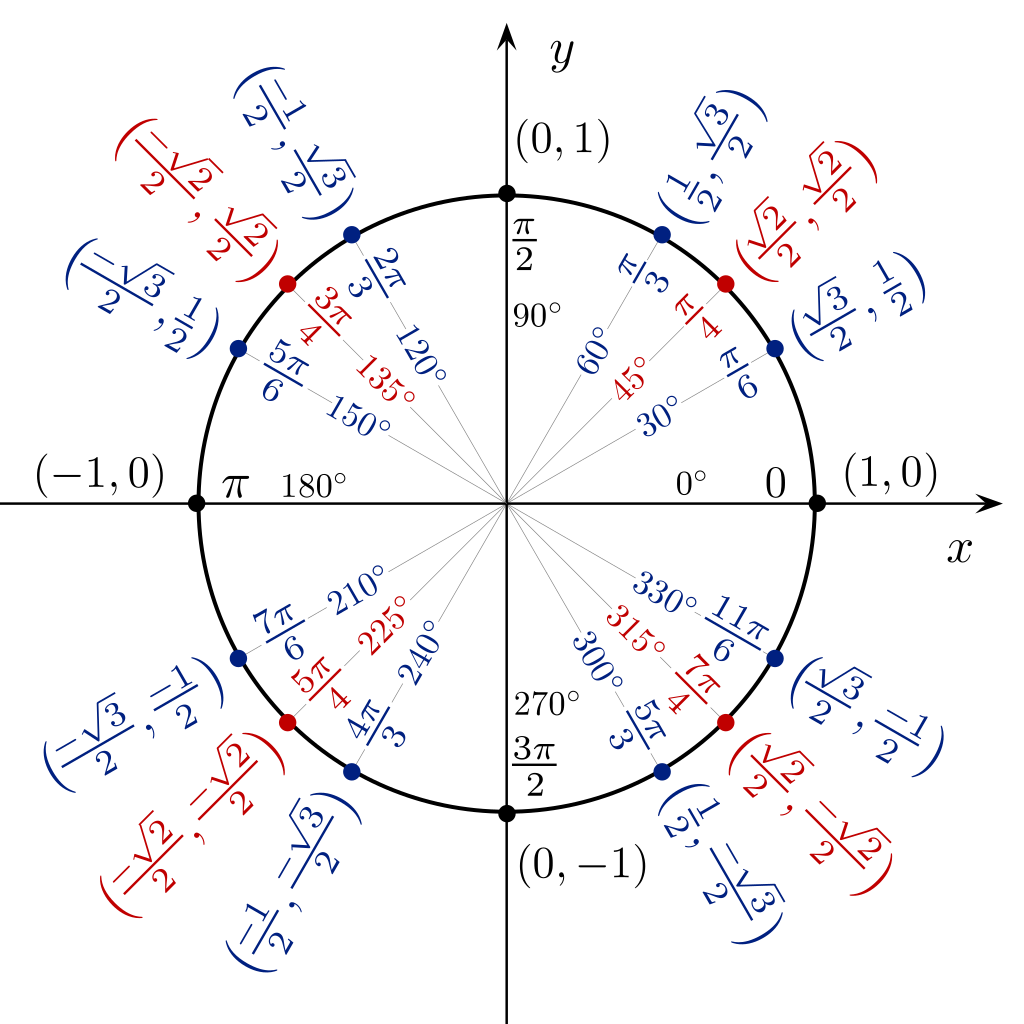
\includegraphics[width=\textwidth]{figures/1024px-Unit_circle_angles_color_svg.png}
\chapter{Boring stuff}
\section{Version History}
\begin{description}
\item[v 0.1 2016:] This project is begun in a trio of physical exercise books as \textit{The Little Book of Physics Formulae}, \textit{The Little Book of Mathematics Formulae}, and \textit{The Little Book of Astronomy Formulae}
\item[v 0.6 2016:] The process of transferring the formulae from paper to LaTeX is initiated, but abandoned (or drifted away from).
\item[v 0.7 2018-03-20:] The project is resurrected (probably because the author started MRes), uploaded to Overleaf, and cleaned up.
\item[v 0.8 2018-07-12:] Remaining formulae imported from the original books.
\item[v 0.9 2018-07-26:] Further formulae imported from undergrad formula sheets.
\item[v 1.0 2018-07-28:] First public release, with some additions from 0.9.
\item[v 1.0.1 2018-07-31:] Minor corrections, added "dynamical timescale" (2.2.2) and some more formulae to the Statistics chapter (it was looking a little bare).
\item[v 1.1 xxxx:] Font change; added Planck units and some other miscellaneous units to Units of Measurement; fine structure constant to Physical Constants (why wasn't it already there?); stellar luminosity; formulae for Green's functions and other differential equation techniques; minor corrections; Gaussian distributions to Statistics section.
\end{description}

\section{Licensing}

\doclicenseThis
    
(Basically, as long as you credit me and share under a similar license, feel free to use this however you want)

\section{Contact}
    	
Visit www.webofworlds.net for science fiction, science fact, geeky opinions, and maybe some Python code. \\ 
Suggestions or corrections are welcome at webofworlds@gmail.com

\section{Credits}

\begin{description}
\item [Formula Sheets: Audrey Markowskei, ] 
\item [Unit Circle:] By Jim.belk [CC BY-SA 3.0 (https://creativecommons.org/licenses/by-sa/3.0) or GFDL (\url{http://www.gnu.org/copyleft/fdl.html})], from Wikimedia Commons (\url{https://commons.wikimedia.org/wiki/File:Unit_circle_angles_color.svg})
\item [Periodic Table:] By Dmarcus100 [CC BY-SA 4.0 (\url{https://creativecommons.org/licenses/by-sa/4.0})], from Wikimedia Commons (\url{https://commons.wikimedia.org/wiki/File:Periodic_Table_Of_Elements_Atomic_Mass_Black_And_White.jpg})
\end{description}

\newgeometry{left=1cm,top=1cm,bottom=0cm} 
\newpage
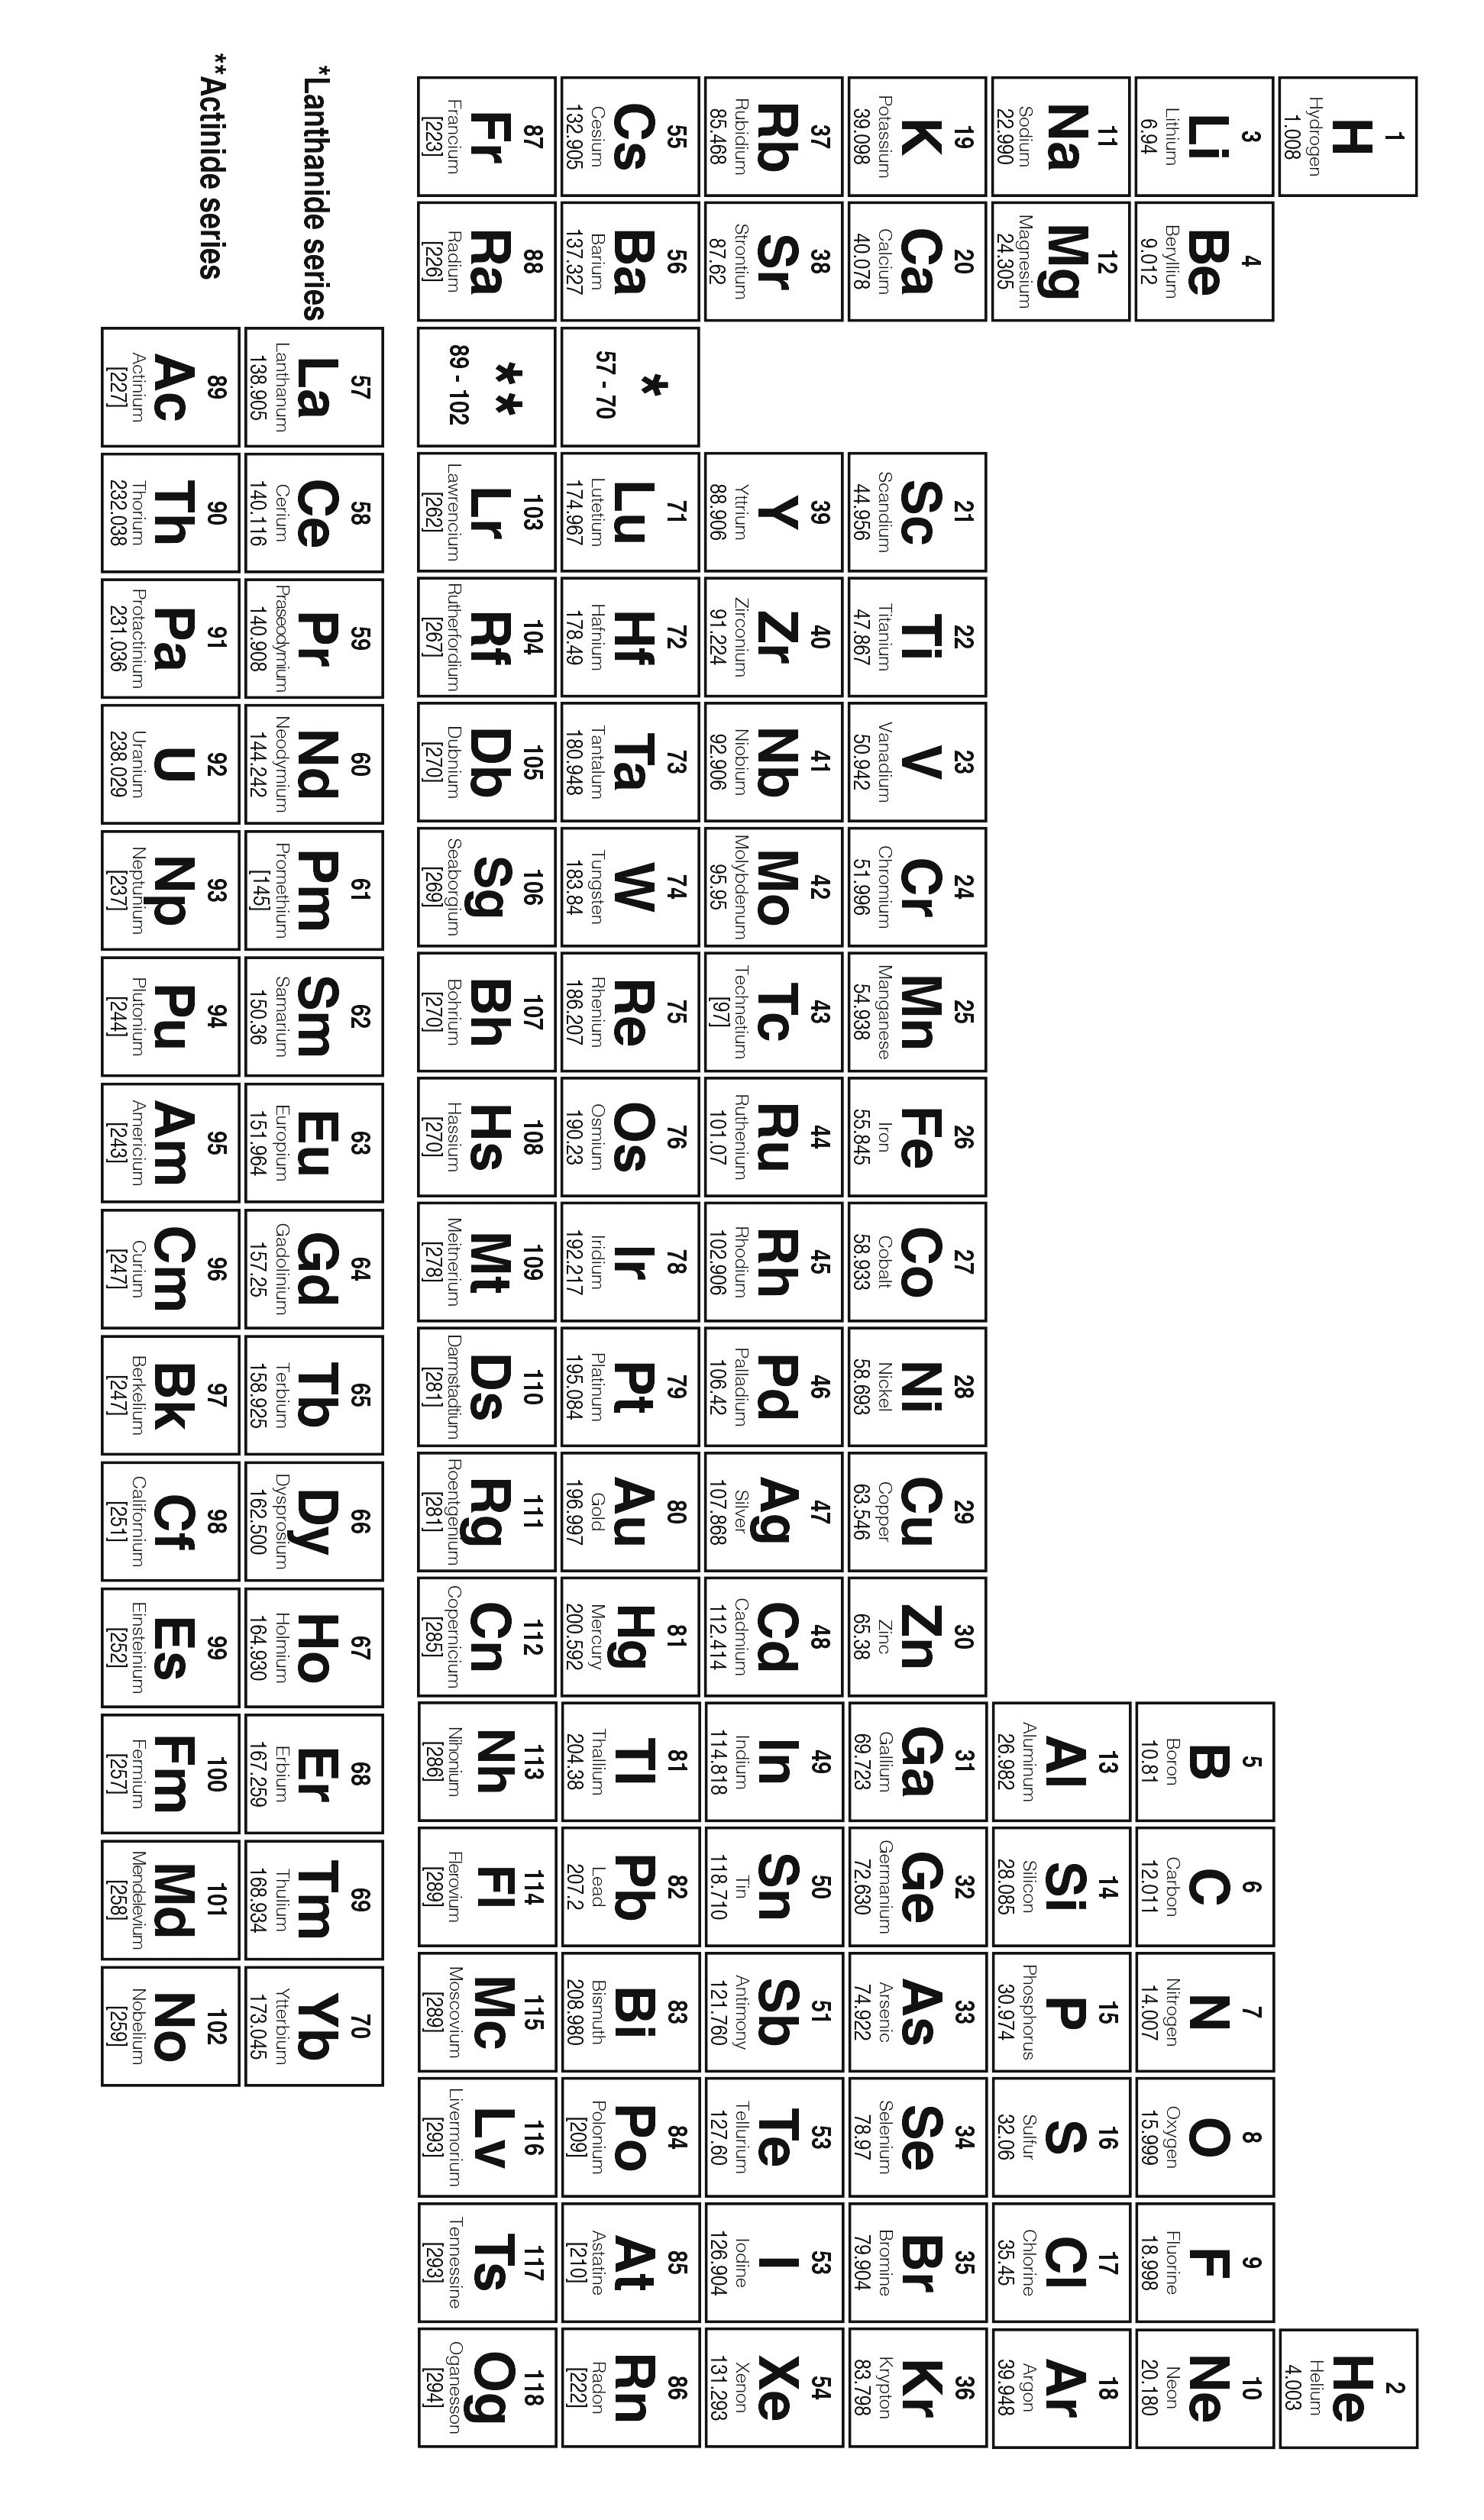
\includegraphics[]{figures/Periodic_Table_Of_Elements_Atomic_Mass_Black_And_White.jpg}
\restoregeometry
\newpage

%\chapter{Other Useful Information}
%\section{Periodic Table of the Elements}

\end{document}
